%
%
% UCSD Doctoral Dissertation Template
% -----------------------------------
% https://github.com/ucsd-thesis/ucsd-thesis
%
%
% ----------------------------------------------------------------------
% WARNING:
%
%   This template has not endorced by OGS or any other official entity.
%   The official formatting guide can be obtained from OGS.
%   It can be found on the web here:
%   http://grad.ucsd.edu/_files/academic-affairs/Dissertations_Theses_Formatting_Manual.pdf
%
%   No guaranty is made that this LaTeX class conforms to the official UCSD guidelines.
%   Make sure that you check the final document against the Formatting Manual.
%
%   That being said, this class has been routinely used for successful
%   publication of doctoral theses.
%
%   The ucsd.cls class files are only valid for doctoral dissertations.
%
%
% ----------------------------------------------------------------------
% GETTING STARTED:
%
%   Lots of information can be found on the project wiki:
%   http://code.google.com/p/ucsd-thesis/wiki/GettingStarted
%
%
%   To make a pdf from this template use the command:
%     pdflatex template
%
%
%   To get started please read the comments in this template file
%   and make changes as appropriate.
%
%   If you successfully submit a thesis with this package please let us
%   know.
%
%
% ----------------------------------------------------------------------
% KNOWN ISSUES:
%
%   Currently only the 12pt size conforms to the UCSD requirements.
%   The 10pt and 11pt options make the footnote fonts too small.
%
%
% ----------------------------------------------------------------------
% HELP/CONTACT:
%
%   If you need help try the ucsd-thesis google group:
%   http://groups.google.com/group/ucsd-thesis
%
%
% ----------------------------------------------------------------------
% BUGS:
%
%   Please report all bugs at:
%   https://github.com/ucsd-thesis/ucsd-thesis/issues
%
%
% ----------------------------------------------------------------------
% More control of the formatting of your thesis can be achieved through
% modifications of the included LaTeX class files:
%
%   * ucsd.cls    -- Class file
%   * uct10.clo   -- Configuration files for font sizes 10pt, 11pt, 12pt
%     uct11.clo
%     uct12.clo
%
% ----------------------------------------------------------------------



% Setup the documentclass
% default options: 12pt, oneside, final
%
% fonts: 10pt, 11pt, 12pt -- are valid for UCSD dissertations.
% sides: oneside, twoside -- note that two-sided theses are not accepted
%                            by OGS.
% mode: draft, final      -- draft mode switches to single spacing,
%                            removes hyperlinks, and places a black box
%                            at every overfull hbox (check these before
%                            submission).
% chapterheads            -- Include this if you want your chapters to read:
%                              Chapter 1
%                              Title of Chapter
%
%                            instead of
%                              1 Title of Chapter
\documentclass[12pt,chapterheads]{ucsd}



% Include all packages you need here.
% Some standard options are suggested below.
%
% See the project wiki for information on how to use
% these packages. Other useful packages are also listed there.
%
%   http://code.google.com/p/ucsd-thesis/wiki/GettingStarted



%% AMS PACKAGES - Chances are you will want some or all
%    of these if writing a dissertation that includes equations.
%  \usepackage{amsmath, amscd, amssymb, amsthm}

%% GRAPHICX - This is the standard package for
%    including graphics for latex/pdflatex.
\usepackage{scrextend}
\usepackage{pslatex}
\usepackage{graphicx}

%% CAPTION
% This overrides some of the ugliness in ucsd.cls and
% allows the text to be double-spaced while letting figures,
% tables, and footnotes to be single-spaced--all OGS requirements.
% NOTE: Must appear after graphics and ams math
\makeatletter
\gdef\@ptsize{2}% 12pt documents
\let\@currsize\normalsize
\makeatother
\usepackage{setspace}
\doublespace
\usepackage[font=small, width=0.9\textwidth]{caption}

%% SUBFIG - Use this to place multiple images in a
%    single figure.  Subfig will handle placement and
%    proper captioning (e.g. Figure 1.2(a))
% \usepackage{subfig}

%% TIMES FONT - replacements for Computer Modern
%%   This package will replace the default font with a
%%   Times-Roman font with math support.
% \usepackage[T1]{fontenc}
% \usepackage{mathptmx}

%% INDEX
%   Uncomment the following two lines to create an index:
% \usepackage{makeidx}
% \makeindex
%   You will need to uncomment the \printindex line near the
%   bibliography to display the index.  Use the command
% \index{keyword}
%   within the text to create an entry in the index for keyword.
%   To compile a LaTeX document with an index the 'makeindex'
%   command will need to be run.  See the wiki for more details.

%% HYPERLINKS
%   To create a PDF with hyperlinks, you need to include the hyperref package.
%   THIS HAS TO BE THE LAST PACKAGE INCLUDED!
%   Note that the options plainpages=false and pdfpagelabels exist
%   to fix indexing associated with having both (ii) and (2) as pages.
%   Also, all links must be black according to OGS.
%   See: http://www.tex.ac.uk/cgi-bin/texfaq2html?label=hyperdupdest
%   Note: This may not work correctly with all DVI viewers (i.e. Yap breaks).
%   NOTE: hyperref will NOT work in draft mode, as noted above.
% \usepackage[colorlinks=true, pdfstartview=FitV,
%             linkcolor=black, citecolor=black,
%             urlcolor=black, plainpages=false,
%             pdfpagelabels]{hyperref}
% \hypersetup{ pdfauthor = {Your Name Here},
%              pdftitle = {The Title of The Dissertation},
%              pdfkeywords = {Keywords for Searching},
%              pdfcreator = {pdfLaTeX with hyperref package},
%              pdfproducer = {pdfLaTeX} }
% \urlstyle{same}
% \usepackage{bookmark}


%% CITATIONS
% Sets citation format
% and fixes up citations madness
\usepackage{microtype}  % avoids citations that hang into the margin


%% FOOTNOTE-MAGIC
% Enables footnotes in tables, re-referencing the same footnote multiple times.
\usepackage{footnote}
\makesavenoteenv{tabular}
\makesavenoteenv{table}


%% TABLE FORMATTING MADNESS
% Enable all sorts of fun table tricks
\usepackage{rotating}  % Enables the sideways environment (NCPW)
\usepackage{array}  % Enables "m" tabular environment http://ctan.org/pkg/array
\usepackage{booktabs}  % Enables \toprule  http://ctan.org/pkg/array


\usepackage[utf8]{inputenc} % Required for inputting international characters
\usepackage[T1]{fontenc} % Output font encoding for international characters

\usepackage{mathpazo} % Use the Palatino font by default
\usepackage{amsmath}
\setcounter{secnumdepth}{4}

\usepackage{mathrsfs}
\newcommand{\Loss}{\mathscr{L}}

\usepackage{dsfont}
\newcommand{\indicator}{\mathds{1}}

\usepackage{amsmath}


\usepackage{xcolor,colortbl}
\newcommand{\mc}[2]{\multicolumn{#1}{c}{#2}}
\definecolor{Gray}{gray}{0.85}
\definecolor{LightCyan}{rgb}{0.88,1,1}
\definecolor{Salmon}{rgb}{1.00, .664, .703}
\definecolor{LightGreen}{rgb}{.484, 1.00, .62}
\definecolor{Tan}{rgb}{1.00, .83, .484}


\newcommand\tab[1][1cm]{\hspace*{#1}}


\usepackage[backend=bibtex,natbib=true]{biblatex} % Use the bibtex backend with the authoryear citation style (which resembles APA)

\addbibresource{main.bib} % The filename of the bibliography

\begin{document}

%% FRONT MATTER
%
%  All of the front matter.
%  This includes the title, degree, dedication, vita, abstract, etc..
%  Modify the file template_frontmatter.tex to change these pages.
%
%
% UCSD Doctoral Dissertation Template
% -----------------------------------
% http://ucsd-thesis.googlecode.com
%
%


%% REQUIRED FIELDS -- Replace with the values appropriate to you

% No symbols, formulas, superscripts, or Greek letters are allowed
% in your title.
\title{Empowering Conservation through Deep Convolutional Neural Networks}

\author{Matthew Epperson}
\degreeyear{\the\year}

% Master's Degree theses will NOT be formatted properly with this file.
\degreetitle{Masters of Science}

\field{Electrical and Computer Engineering}
\specialization{Intelligent Systems, Robotics, and Controls}  % If you have a specialization, add it here

\chair{Nikolay Atanasov}
% Uncomment the next line iff you have a Co-Chair
% \cochair{Professor Cochair Semimaster}
%
% Or, uncomment the next line iff you have two equal Co-Chairs.
%\cochairs{Professor Chair Masterish}{Professor Chair Masterish}

%  The rest of the committee members  must be alphabetized by last name.
\othermembers{
Ryan Kastner\\
Curt Schurgers\\
}
\numberofmembers{3} % |chair| + |cochair| + |othermembers|


%% START THE FRONTMATTER
%
\begin{frontmatter}

%% TITLE PAGES
%
%  This command generates the title, copyright, and signature pages.
%
\makefrontmatter

%% DEDICATION
%
%  You have three choices here:
%    1. Use the ``dedication'' environment.
%       Put in the text you want, and everything will be formated for
%       you. You'll get a perfectly respectable dedication page.
%
%
%    2. Use the ``mydedication'' environment.  If you don't like the
%       formatting of option 1, use this environment and format things
%       however you wish.
%
%    3. If you don't want a dedication, it's not required.
%
%
\begin{dedication}
  To my parents who have always believed in me even when I didn't believe in myself
\end{dedication}

%% SETUP THE TABLE OF CONTENTS
%
\tableofcontents
\listoffigures  % Comment if you don't have any figures
\listoftables   % Comment if you don't have any tables


%% ACKNOWLEDGEMENTS
\begin{acknowledgements}
Thanks to my wonderful committee that made this thesis possible! It's been a whirlwind ride and I'm grateful to have been able to complete a thesis with three awesome professors!

Thanks to Dr. Kastner and Dr. Curt Schurgers for welcoming me into Engineers for Exploration during my first year. The program has allowed me to embrace two of my greatest passions in life! Thanks to Eric Lo and the other E4E members who were a part of this project.

I would also like to thank Professor Jamie Rotenberg from University of North Carolina Wilmington for supporting the Belize expedition! Without you this thesis would not have been possible. Looking forward to continuing to work together and hopefully meeting in person someday!

\end{acknowledgements}


%% ABSTRACT
%
%  Doctoral dissertation abstracts should not exceed 350 words.
%   The abstract may continue to a second page if necessary.
%
\begin{abstract}

Aerial imagery presents conservationists and ecologists a powerful tool for noninvasive monitoring of ecosystems and wildlife. The two traditional methods for collecting aerial imagery, manned aircraft and satellites, are tremendously expensive and can suffer from poor resolution or obstruction by weather. Unmanned aerial systems (UAS) present conservationists and ecologists a flexible tool for collecting high resolution imagery at a fraction of the price. In this thesis we asked: Can we take advantage of the sub-meter, high-resolution imagery to detect specific tree species or groups, and use these data as indicators of rainforest functional traits and characteristics? We demonstrate a low-cost method for obtaining high-resolution aerial imagery in a rainforest of Belize using a drone over three sites in two rainforest protected areas. We built a work flow that uses Structure from Motion (SfM) on the drone images to create a large orthomosaic and a Deep Convolutional Neural Network (CNN) to classify indicator tree species. We selected: 1) Cohune Palm (Attalea cohune) as they are indicative of past disturbance and current soil condition; and, 2) the dry-season deciduous tree group since deciduousness is an important ecological factor of rainforest structure and function. This framework serves as a guide for tackling difficult ecological challenges and we show two additionally examples of how a similar architecture can help count wildlife populations in the Antarctic.

\end{abstract}


\end{frontmatter}






%% DISSERTATION

% A common strategy here is to include files for each of the chapters. I.e.,
% Place the chapters is separate files:
%   chapter1.tex, chapter2.tex
% Then use the commands:
% Chapter 1

\chapter{Introduction} % Main chapter title

\label{Chapter1} % For referencing the chapter elsewhere, use \ref{Chapter1}

%----------------------------------------------------------------------------------------

% Define some commands to keep the formatting separated from the content
\newcommand{\keyword}[1]{\textbf{#1}}
\newcommand{\tabhead}[1]{\textbf{#1}}
\newcommand{\code}[1]{\texttt{#1}}
\newcommand{\file}[1]{\texttt{\bfseries#1}}
\newcommand{\option}[1]{\texttt{\itshape#1}}

%------------------------------------------------------------------
%------------------------------------------------------------------

\section{Background}

Computer Vision (CV) has jumped by leaps and bounds in the last five years as machine learning, notably deep convolutional neural networks, have become a driving force for pushing the bounds on tasks such as classification, segmentation, and object detection. Industry has jumped on the deep learning wave and today you can purchase products which use facial recognition for security, ride in vehicles that operate autonomously in complex safety critical environments, or get a cancer diagnosis more accurate then seasoned doctors from a machine \cite{Cancer}.

In parallel to advances in computer vision micro-UAVs, colloquially referred to as drones, have found there way out of research labs and into the hands of consumers and professions a like. As demand for drones has built we have seen a steady increase in capabilities with regards to stability, vehicle configuration, flight duration, payload options and autonomy.

One area that is consistently under served by emerging technologies are ecology and conservation. Both areas have ample need for these technologies which can enable scientists access to the information needed to gain new insights into complex environments that are seeing rapid change due to climate change and habitat loss. In this research we show a pipeline see ~\ref{fig:Pipeline} for collecting very high resolution aerial imagery from UAVs, pre-processing the imagery into an orthomosaic using commercial GIS software, and finally using deep convolution neural networks to accurately identify individual species of trees in rain forest canopies. We show that this fine grained classification is only possible with superior than satellite resolution and it has the ability to generalize to new sites with different lighting conditions and resolutions. This study directly enabled ecologists to pull useful insights from our study area.

\begin{figure}[ht]
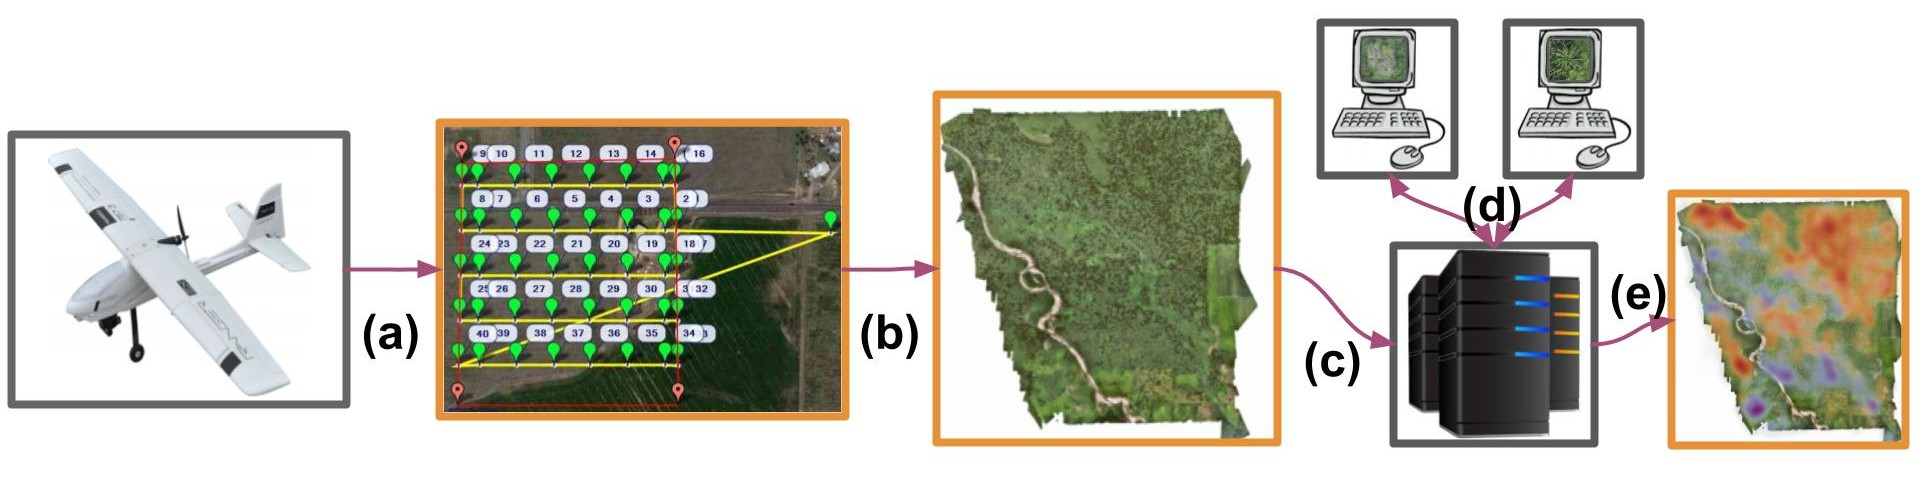
\includegraphics[width=1.0\textwidth]{Figures/Pipeline.jpg}
\caption{\textbf{Data Processing Pipeline.} a) UAV flies a lawn mower flight pattern taking pictures at regular intervals. b) The raw images with GPS and orientation information are stitched together to create an orthomosaic of the canopy; covering about 8.73km2 of data at the BFREE site. c) Orthomosaic is split into smaller images and stored on a server for labeling. d) Web based tool distributes a small subset of the images to volunteers who label them to provide “ground truth”. e) CNN uses the ground truth data train a classifier to detect ecological features (e.g., a specific type of tree). This classifier is used to process the remaining data and automatically characterize the images and orthophoto.}
\label{fig:Pipeline}
\end{figure}

%------------------------------------------------------------------
%------------------------------------------------------------------

\section{What is Deep Learning?}

Deep Learning is an aspect of machine learning that is currently very popular for a variety of tasks, such as natural language processing, computer vision, and even control. Traditionally for each of these disciplines researchers would posit a model that tried to capture the underlying truth of how the world works. For natural language processing this might be how consonants and vowels are related to each other; how different parts of a sentence are connected and influence the overall semantic meaning. For computer vision it might be how edges, contours or colors make up an object such as a dog or cat. For the most part these largely hand designed models fail to capture the entire underlying model which might be highly nonlinear in nature.

This is where neural networks step in as universal function approximaters. Neural networks are formed by an input layer, hidden layer(s), and an output layer. Each node is like a neuron and is connected to other nodes much like the synapses of biological systems. The systems are trained by providing training examples and comparing the output with the desired output and then performing back-propagation to push the parameters of the network towards a better solution. The upshot of these networks are that they are model free reducing the burden on the engineer or scientist to create one by hand. The downside is that they often require massive amounts of data before they perform well, can be computationally expensive, and are largely black boxes that are difficult to inspect. For computer vision the most popular deep learning algorithm has been convolutional neural networks (CNN) which we will utilize as powerful tool for automating perception tasks in ecology and conservation.

\subsection{Brief background to CNNs}

Using computer algorithms to detect and classify objects in digital images is an intrinsically hard problem that has eluded computer vision experts best attempts to model for years. Retaining the 2D structure of an object in an image and discerning how semantic parts of it relate to each other in any given orientation or position is no small feat.

A big step forward came in 2012 when Alex Krizhevsky proposed a learning algorithm that is loosely inspired by how the human visual cortex system works \cite{AlexNet}. It uses many stacked layers of 2D convolutional filters along with nonlinear activation layers to form a neural network capable of learning complex hierarchical representations of objects. While the idea itself wasn't novel idea (neural networks have been around for decades) his use of the massively parallel computation available in graphic processing units (GPUs), deeply stacked layers, and massive amounts of training data allowed him to score $10.8\%$ better than the nearest computation; a huge break through in accuracy. Krizhevsky’s neural network called “AlexNet” is largely considered a silver bullet that helped computer vision researchers overcome a barrier in classification accuracy that they had been running up against for years and leading to a overall boom in deep learning research.

CNNs are a very active area of research and at this point AlexNet is considered outdated. Today Residual network (ResNet) \cite{ResNet} and Densely Connected Convolutional Networks (DenseNet) \cite{DenseNet} are the top performing networks that form the backbone for other problems like object detection, segmentation, and pose regression.

\subsection{Object Detection}

A subset of Deep Learning networks for computer vision are called object detectors. These networks deal with not only classifying an image, but first localizing an individual object in an image frame before assigning it a classification as well as a confidence. Many open source variants of object detectors exist with various strengths and weakness. We considered two algorithms for object detection and recognition: Faster-RCNN and YOLOv2. Faster-RCNN \cite{FASTER-RCNN} uses two networks where the first network proposes a “region” while the second network classifies that region.  YOLOv2 \cite{YOLOv2} uses a single unified network that simultaneously predicts location and class. They both use open source GPU frameworks Caffe and Darknet respectively.  While the two networks are comparable in accuracy on standard datasets, we found that YOLOv2 had the advantage when working with high resolution imagery as it can accept arbitrarily large input images. This is unlike many neural networks where the input size is fixed and makes detection of small objects in high resolution imagery harder due downsampling an image before passing it through the network.

%------------------------------------------------------------------
%------------------------------------------------------------------

\section{Why Ecology and Conservation?}

Macro understanding of ecosystems are usually done by making assumptions based on \textit{macro} features instead of fine grained details. For example forests are usually classified into broads types: coniferous, evergreen, tropical, or mediterranean instead of the individual species that make up the forest. Population counts of arctic fur seals are done with boots on the ground. Coral reef classification is done exhaustively by hand on only small sections at a time. The more fine grain the examination the more labor intensive the process which leads to a loss in temporal coherence as such tasks are only performed rarely and at much greater cost. Ideally researchers would be able to obtain fine-grain temporally coherent analysis of ecosystems without having to invest large amounts of time and money. This is where computer vision can jump in.

\subsection{What does Computer Vision offer Ecologists?}

A few tasks that researchers need to perform such as counting populations of individuals species, marking geographical distribution of individuals, or even identification of individuals in a population are quite easy for humans but traditionally very difficult to automate with machines. The promise and hype around much of the capabilities surrounding deep learning is underlied by the idea that given enough training data we can teach machines to operate at and even above human level abilities for certain tasks. Applying these emerging technologies can allow researchers to automate many processes that can be too labor intensive to do manually.

This technology has already begun to seep into conservation projects. For example Right Whale classification and individual IDing was presented in Kaggle competition by NOAA \cite{DeepSense}. In a similar sense the authors of \cite{Gorilla} used an object detector with facial recognition to find and ID gorillas in the wild. The authors in \cite{GoogleTrees} leveraged Google Street View and Google Earth satellite imagery to classify trees, geo-locate them, and estimate trunk thickness. Researchers from both engineering and ecology are just beginning to jointly explore computer vision tools for these types of challenging tasks.

%------------------------------------------------------------------
%------------------------------------------------------------------

\section{Why UAVs?}

Taking to the sky has always been a force multiplier for mankind and few things have put flight into peoples hands as cheaply as micro unmanned aerial vehicles which we will interchangeable call UAVs, MAVs, or drones. In the consumer world UAVs are more commonly referred to as drones and come in a price range from sub fifty dollar toys designed to be flown inside by children to multi-thousand dollar aircraft for taking action videos. They have been successfully commercialized and used by government organizations to: survey land, create 3D reconstructions of building, monitor agricultural crops, perform remote inspection on wind turbines, assistant in search and rescue, and even provide broadband coverage during natural disasters to name a few.

\subsection{Types of UAVs}

The two most common platforms are multi-rotor copters and fixed wing planes.

Multi-rotor copters usually consist of three to eight propellers, commonly four (quadcopters), with battery, electronics and payload centered on the vehicle. They range in size from as small as ten centimeters to several meters for the largest platforms. Their popularity comes from their ability to move in six degrees of freedom and their ease of flying; making it an ideal platform for inspection and shooting video. They aren't very aerodynamically efficient and usually have flight durations ranging from 10-45 minutes depending on configuration and payload. They are often very weight constrained limiting the types and sizes of payloads they are capable of carrying.

Fixed wing planes are essentially miniaturized versions of manned planes we are accustomed to seeing in our skies. Just like traditional aircraft they come in a large variety of shapes and sizes that have different advantages in flight duration, agility, payload capacity, etc... They vary from hand launched, to shot runway takeoffs, to being catapulted by pneumatic machines. The advantage to fixed wing aircraft are that they are much more efficient than multi-rotor copters with increased payload capacity, longer flight durations, and faster speeds.

For conservation in ecology both vehicle types have important use cases. For our research focusing on wide-scale classification of rain forest canopies a fixed wing aircraft was a natural choice for its long range capabilities.

\subsection{Autopilots}

At the heart of most MAVs are highly sophisticated autopilot systems that use inertial measurement units, GPS, and embedded processors capable of handling low level control/stabilization as well as high level decision making. Prior to a decade ago autopilots with these capabilities were extremely expensive and not commercially available. As cheap micro electronic measurement sensors (MEMS) and faster embedded processors made their way onto the market they began to find their way into autopilots. This is at the heart of the explosion of UAVs on the market. Today they are many autopilots with many available as open source, open hardware projects which are ideal for research applications.

Autopilots usually operate in two different modes: fully autonomous and fly-by-wire. In fly-by-wire mode the autopilot sits between the human and the aircraft to stabilize the vehicle and make the end task for the human much easier. All multi-rotor vehicles operate in this manner. In fully autonomous mode the vehicle has a high level mission plan from the user which commonly consists of a set of waypoints and actions to perform at those waypoints. In this research we make heavy use of this waypoint following to automate the flight paths and image capture in order to achieve a certain amount of overlap per image.

\subsection{What do UAVs offer Conservationists?}

% Chapter 2

\chapter{Convolutional Neural Networks} % Main chapter title

\label{Chapter2}

%-------------------------------------------------------------------------------
%-------------------------------------------------------------------------------

\section{CNNs: Layer by Layer}

Convolutional neural networks have been very successful in computer vision as their key ingredient convolution filters preserve 2D structure and are able to pull features from images. Back propogation and stochastic gradient descent are used to optimize these filters in order to produce. Here I will cover some of the most common layers used in CNNs.

\subsection{Convolution Layer}

The first and foremost layer is the convolution layer. A convolution layer contains a set of filters which are \textit{convolved} across feature maps in order to get the feature map. Let's take a concrete look at what this means. Imagine we are working with images that are of the shape 28x28x3 pixels. We then decide we want to use a convolution filter of size 2x2x5 which will result in a 28x28x5 feature map. Each kernel in this filter will be of size 2x2x3 since the depth in our original image is 3 and there will be five kernels. We then take the dot product of each slice in our 2x2x3 matrix against the original image at pixel 0x0 giving us 3 scalar values which are summed to get the first value in the first feature map of the output. We then slide these filters across the entire feature map in x and y thereby creating a new feature map.  See ~\ref{fig:Convolution} for an example of convolving two 3x3x3 kernels on a 7x7 image.  A few things to consider when sliding the feature maps are image padding. For pixel 0,0 in our example part of the filter would be off the image. To keep the convolution consistent people will often times pad the edges of the image with 0 or 0.5. Additionally a stride length can be set which determines how far we move the filter at each step. A stride length of 2 would skip every other pixel when sliding.

\begin{figure}[ht]
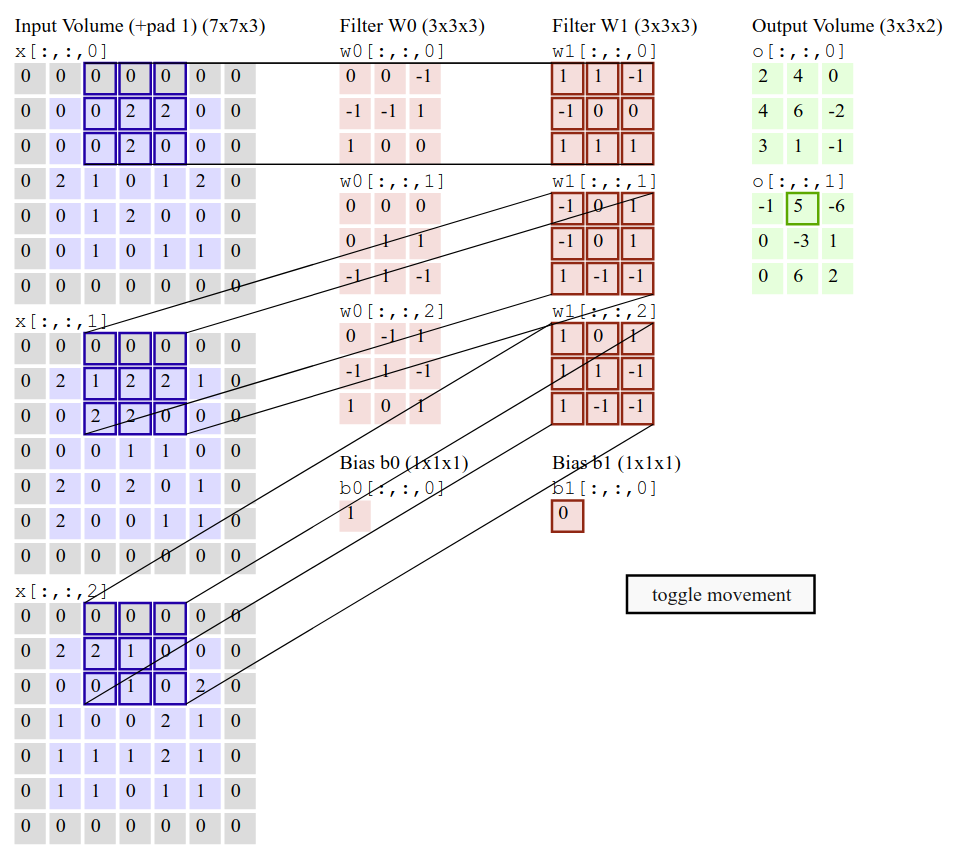
\includegraphics[width=0.9\textwidth]{Figures/Convolution.png}
\caption{An example of performing a 3x3 convolution with a depth of two on an 7x7x3 image with 1 pixel of padding from Andrej Karpathy's Stanford CNN Course \cite{StanfordConv}}
\label{fig:Convolution}
\end{figure}

\subsection{Activation Layer}

Its common after each of the convolutional layers to apply a non-linear activation function. A few examples of activation include: \\

\[ \sigma(x) = \frac{1}{1+e^{-x}} \]
\[ \tanh(x) = \frac{e^x - e^{-x}}{e^x + e^{-x}} \]

\[ ReLu(x) = \begin{cases}
      0 & x < 0 \\
      x & x \geq 0
   \end{cases}
\]

ReLu or rectified linear unit has been a popular choice for cnns as it is computation efficient without sacrificing accuracy.

\subsection{Pooling Layer}

Pooling layers are used to downsample feature maps from layer to layer. Two common flavors of pooling layers are max pooling and average pooling. Max pooling simply looks at a window and returns only the maximum value. Average pooling as it names suggests averages all the values in the window and returns that value. Lets take for example a 2x2 max pooling layer with an feature map of size of 128x128x32. After applying the pooling layer we would have 64x64x32 as an output. A common intuition behind max pooling is that it provides spatial invariance, i.e. if an object shifts by a few pixels we will still have a high response. An alternative to max pooling is using strided convolutions. The argument for this is that a good amount of information is lost in pooling layers.

\subsection{Fully Connected Layer}

Fully connected layers are what we traditional think of as the multi-layer perceptron model. They are commonly used in the final layer of CNNs to distill feature maps from a multi-dimensional matrix into a vector that can be then used for classification or regression. As a simple example are classification networks that will use two fully connected layers where the output is a vector of the same length as number of classes they want to predict from. SoftMax is applied to the vector to normalize the sum of the vector to one and then each scalar in the vector is interpreted as a likelihood of that image being of that particular class.

\subsection{Transfer Learning}

Transfer learning is the process of taking a neural network trained for a certain task and refining it for another. A common example of this is retraining a classification network to predict a different set of classes than what it was originally trained for or changed from a classifier to a regression network. The common intuition for this is that the early layers in the network have learned basic features like, curves, corners, or other simple patterns that are universal in all types of objects. The top layers which carry the strong semantic information are closer to the end and therefore receive more gradient during back propagation. Some methods even freeze the weights for lower levels as fixed feature extractors and only allow the the final layers to change during training. As a bonus, transfer learning reduces the total time to train a network as the lower levels of a network take longer to train that the deeper layers.

When exploring new architectures it is common procedure to simply download a set of weights for a popular network backbone and just apply transfer learning from there. In these next sections I will cover some of the popular network backbones.

\subsection{VGG16}

VGG16 was one of the first major networks after AlexNet which went for simplicity and depth \cite{VGG16}. The first contribution was its simplicity. CNNs before VGG used very large filter sizes, for example AlexNet used 11x11, which led to large parameter sizes. The authors of VGG16 instead used series of two back to back convolution/ReLu layers with 3x3 filters before doing max pooling. VGG16 at the time was considered a very deep network with 13 convolution layers and 3 fully connected layers. It showed that very deep networks were extremely important in learning the hierarchical features necessary for good classification. VGG16 scored $7.3\%$ error rate on ImageNet dataset.

\subsection{ResNet}

In 2015 Microsoft Research came out with \textit{Deep Residual Learning for Image Recognition} \cite{ResNet} which had 152 layers and new type of of block called the residual block. It scored $3.6\%$ on the ImageNet challenge in 2015. A residual block is a normal feed forward neural network that adds in \textit{shortcut} connections where the input to a layer is both fed through a layer but also routed around the layer and added to the output of the next layer. See ~\ref{fig:ResBlock} for a visual description. They hypothesized that a residual mapping induced by this block would be easier to learn than the original feed-forward network. ResNets come in several popular forms now such as ResNet18, ResNet32, ResNet50, ResNet101, and ResNet152, where the choice of depth is based on computational resources and dataset. Most popular deep learning frameworks have pretrained ResNet models available for download.

Another intuition behind ResNets success is that the \textit{shortcut} connections allow gradients to move more easily through the network which helps alleviate a problem known as the vanishing gradient. Vanishing gradients is the problem where the loss at the end of the network has very little impact on changing the weights on the earlier layers and was one of the main reasons preventing networks from going as deep as ResNet. In the next network the use of skip connection is taken even further.

\begin{figure}[ht]
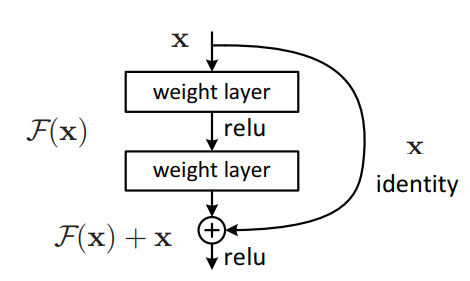
\includegraphics[width=0.9\textwidth]{Figures/ResBlock.png}
\caption{Diagram of Residual Block from \cite{ResNet}}
\label{fig:ResBlock}
\end{figure}

\subsection{DenseNet}

In 2016 Densely Connected Convolutional Networks (DenseNets) were proposed and shown to match and beat the residual network architecture on many datasets while using much fewer parameters and therefore computation. With DenseNets the authors connect all feature maps of same size together through concatenation so that the lth layer will have (l-1) feature maps. This is different then the ResNet model which uses summation in its shortcut connections. In order to concatenate feature maps across max pooling layers DenseNet introduce transition layers. These transition layers pass the prior feature maps through batch normalization, convolution, and finally average pooling before concatenating them to layers further down.

\begin{figure}[ht]
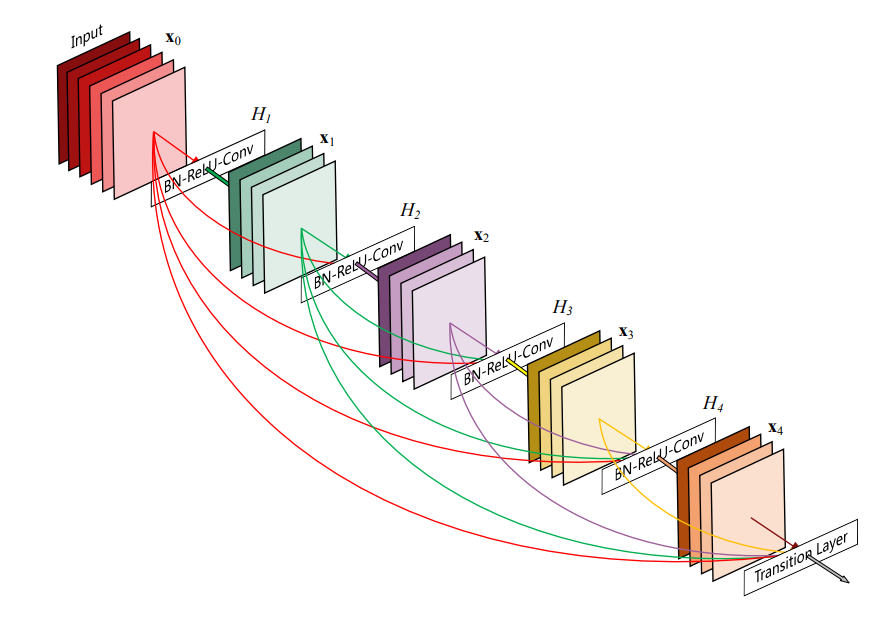
\includegraphics[width=0.9\textwidth]{Figures/DenseNet.png}
\caption{Diagram of Residual Block from \cite{DenseNet}}
\label{fig:DenseNet}
\end{figure}

%-------------------------------------------------------------------------------
%-------------------------------------------------------------------------------
\section{Object Detection Networks}

Object detection networks deal with the problem of first localizing an object with an image frame as well as classifying that object and is generally considered a harder problem then pure classification tasks. The two popular datasets for benchmarking results are \textit{Common Objects in Context} (COCO) \cite{COCO} and \textit{The PASCAL Visual Object Classes} (PASCAL VOC) \cite{VOC}. At the time this work began the two most popular object detection networks were Faster-RCNN and YOLOv2 which I will cover in depth in the next two sections. Since then the state of the art has progressed considerably. Future work might include exploring this architectures.

\subsection{Faster-RCNN}

Faster-RCNN \cite{FASTER-RCNN}, where the R stands for region, is one of the most popular object detection networks at the moment and is an advancement on the authors previous two networks RCNN and Fast RCNN. The authors show results for both VGG16 and ZF network backbones, but many open source implementations of Faster-RCNN have replaced these backbones with various ResNet and DenseNets backbones.

The main contribution of Faster-RCNN is the Region Proposal Network (RPN) which replaces Fast-RCNNs slower, more complicated region proposal mechanism. It works by sliding a window across the final convolution feature map in a network and simultaneously predicting class probability and objectness. Objectness in this context is the probability that there is an object present in the bounding box. The RPN is implemented as a single NxN conv layer that maps into a lower dimension followed by two 1x1 conv layers for class probability and objectness. Furthermore they make use anchor boxes or priors on bounding boxes to make the task of the box regressor easier. At each position in the sliding window there are 9 anchor boxes which the regressor predicts bounding boxes with respect to.

The training scheme for this network is a multi-step process which involves training the RPN and Fast-RCNN networks separately and then later fixing the conv layers of Fast-RCNN and just fine-tuning the RPN.

\subsubsection{Loss}
The loss for Faster-RCNN is split into two parts as shown below.

\begin{align}
    \Loss = \Loss_{cls} +\Loss_{reg}
\end{align}

Given $p_i$ is the predicted confidence that the ith anchor box is an object and $p_i^*$ is a binary indicator that the anchor box has an IoU greater than 0.7 with a ground truth we can define the loss as:

\begin{align}
    \Loss_{cls}(p_i,p_i^*) = \frac{1}{N_{cls}} \sum_{i=1}^{A} [p_i\log(p_i) + (p_i^*-p_i)\log(1-p_i)]
\end{align}

We then parameterize the anchor box and bounding box truth as the following where $_a$ indicates a parameter from the anchor box and $*$ from the ground truth.

\begin{align}
    t_x = \frac{(x - x_a)}{w_a} \\
    t_y = \frac{(y - y_a)}{h_a} \\
    t_w = \log(\frac{w}{w_a}) \\
    t_h = \log(\frac{h}{h_a}) \\
    t_x^* = \frac{(x^* - x_a)}{w_a} \\
    t_y^* = \frac{(y^* - y_a)}{h_a} \\
    t_w^* = \log(\frac{w^*}{w_a}) \\
    t_h^* = \log(\frac{h^*}{h_a}) \\
\end{align}

Next we define the regression loss where again we use $p_i^*$ as an indicator whether this anchor box has an IoU above 0.7 with the ground truth.

\begin{multline}
    \Loss_{reg}(p_i^*, t, t^*) = p_i^*(Smooth_{L1}(t_x-t_x^*) + Smooth_{L1}(t_y-t_y*) \\ + Smooth_{L1}(t_w-t_w*) + SL1(t_h-t_h*)) \\
\end{multline}

\begin{align}
    Smooth_{L1}(d) = \begin{cases}
      0.5d^2 & if |d| \leq 0 \\
      |d| - 0.5 & otherwise
   \end{cases}
\end{align}

\subsection{YOLOv2}

YOLOv2, You Only Look Once, is another successful object detector released in 2016 \cite{YOLOv2}. It's key contribution is a unified network that simultaneously predicts object class and location with out the use of a secondary Region Proposal Network. While maintaining comparable accuracy to Faster-RCNN it runs at a much higher frame rate.

The backbone is of the authors design that uses only 3x3 and 1x1 convolutions, max pooling layers, and batch normalization. The network contains 23 convolution layers, 5 max pooling layers, and one short cut layer that concatenates features from lower levels to the final layer. Since the model contains no fully connected layers the network input size is unconstrained. The 5 max pooling layers of stride 2 mean that the final feature map will have a width and height that is the original width and height divided by $2^5$. As such the the original network input is usually selected to be a multiple of 32 i.e. 320, 416, 608, etc... An example of the network architecture is shown in table~\ref{table:YOLOV2}

\begin{center}
\begin{table}[h]\footnotesize
    \caption{YOLOv2 Network Architecture layer by layer for an input resolution of 608 x 608}\label{table:YOLOV2}
    \begin{tabular}{| l | l | l | l | l |}
    \hline
    layer  & filters & size & input & output \\ \hline \hline

    \rowcolor{LightCyan}
    0 conv & 32 & 3 x 3 / 1 & 608 x 608 x 3 & 608 x 608 x 32 \\ \hline

    \rowcolor{Salmon}
    1 max  & N/A & 2 x 2 / 2 & 608 x 608 x  32   &  304 x 304 x  32 \\ \hline \hline

    \rowcolor{LightCyan}
    2 conv &       64  & 3 x 3 / 1   & 304 x 304 x  32   & 304 x 304 x  64 \\ \hline

    \rowcolor{Salmon}
    3 max &     N/A     & 2 x 2 / 2   & 304 x 304 x  64   &   152 x 152 x  64 \\ \hline \hline

    \rowcolor{LightCyan}
    4 conv &    128  & 3 x 3 / 1   & 152 x 152 x  64   &   152 x 152 x 128 \\ \hline

    \rowcolor{LightCyan}
    5 conv &     64  & 1 x 1 / 1   & 152 x 152 x 128   &   152 x 152 x  64 \\ \hline

    \rowcolor{LightCyan}
    6 conv &    128  & 3 x 3 / 1   & 152 x 152 x  64   &   152 x 152 x 128 \\ \hline

    \rowcolor{Salmon}
    7 max &     N/A     & 2 x 2 / 2   & 152 x 152 x 128   &    76 x  76 x 128 \\ \hline \hline

    \rowcolor{LightCyan}
    8 conv &    256  & 3 x 3 / 1   &  76 x  76 x 128   &    76 x  76 x 256 \\ \hline

    \rowcolor{LightCyan}
    9 conv &    128  & 1 x 1 / 1   &  76 x  76 x 256   &    76 x  76 x 128 \\ \hline

    \rowcolor{LightCyan}
   10 conv &    256  & 3 x 3 / 1   &  76 x  76 x 128   &    76 x  76 x 256 \\ \hline

    \rowcolor{Salmon}
   11 max &     N/A     & 2 x 2 / 2   &  76 x  76 x 256   &    38 x  38 x 256 \\ \hline \hline

    \rowcolor{LightCyan}
   12 conv &    512  & 3 x 3 / 1   &  38 x  38 x 256   &    38 x  38 x 512 \\ \hline

    \rowcolor{LightCyan}
   13 conv &    256  & 1 x 1 / 1   &  38 x  38 x 512   &    38 x  38 x 256 \\ \hline

    \rowcolor{LightCyan}
   14 conv &    512  & 3 x 3 / 1   &  38 x  38 x 256   &    38 x  38 x 512 \\ \hline

    \rowcolor{LightCyan}
   15 conv &    256  & 1 x 1 / 1   &  38 x  38 x 512   &    38 x  38 x 256 \\ \hline

    \rowcolor{LightCyan}
   16 conv &    512  & 3 x 3 / 1   &  38 x  38 x 256   &    38 x  38 x 512 \\ \hline

   \rowcolor{Salmon}
   17 max &     N/A     & 2 x 2 / 2   &  38 x  38 x 512   &    19 x  19 x 512 \\ \hline \hline

    \rowcolor{LightCyan}
   18 conv &   1024  & 3 x 3 / 1   &  19 x  19 x 512   &    19 x  19 x1024 \\ \hline

    \rowcolor{LightCyan}
   19 conv &    512  & 1 x 1 / 1   &  19 x  19 x1024   &    19 x  19 x 512 \\ \hline

    \rowcolor{LightCyan}
   20 conv &   1024  & 3 x 3 / 1   &  19 x  19 x 512   &    19 x  19 x1024 \\ \hline

    \rowcolor{LightCyan}
   21 conv &    512  & 1 x 1 / 1   &  19 x  19 x1024   &    19 x  19 x 512 \\ \hline

    \rowcolor{LightCyan}
   22 conv &   1024  & 3 x 3 / 1   &  19 x  19 x 512   &    19 x  19 x1024 \\ \hline

    \rowcolor{LightCyan}
   23 conv &   1024  & 3 x 3 / 1   &  19 x  19 x1024   &    19 x  19 x1024 \\ \hline

    \rowcolor{LightCyan}
   24 conv &   1024  & 3 x 3 / 1   &  19 x  19 x1024   &    19 x  19 x1024 \\ \hline \hline

   \rowcolor{LightGreen}
   25 route  & 16 & N/A & N/A & N/A \\ \hline

   \rowcolor{Tan}
   26 reorg & N/A &            / 2      & 38 x  38 x 512    &    19 x  19 x2048 \\ \hline

   \rowcolor{LightGreen}
   27 route & 26 & 24 & N/A & N/A \\ \hline \hline

    \rowcolor{LightCyan}
   28 conv &   1024  & 3 x 3 / 1   & 19 x  19 x3072    &    19 x  19 x1024 \\ \hline

    \rowcolor{LightCyan}
   29 conv &     35  & 1 x 1 / 1   & 19 x  19 x1024    &    19 x  19 x  35 \\ \hline

    \hline
    \end{tabular}
\end{table}
\end{center}

YOLOv2 takes a simple approach to bounding box regression and class prediction. To understand how it works lets view the final feature map as a grid. At each location in this grid we want to predict bounding boxes and give a confidence metric for how likely there is to be an object there. We want to predict 5 numbers at each location in the grid plus a confidence for each class as show below:

\begin{align}\label{eq:bbox_regressed}
    t_x,t_y,t_w,t_h,t_o,P(C_1),...,P(C_N)
\end{align}

The parameters $t_x,t_y,t_w,t_h$ are regressed with relation to the feature map x,y location which we call $f_x$ and $f_y$. Further $t_x,t_y$ are constrained to be between [0,1] by the logistic function. We also define $p_w,p_h$ as the prior width and height for the anchor boxes.


\begin{align}
    b_x &= \sigma(t_x) + f_x \\
    b_y &= \sigma(t_y) + f_y \\
    b_w &= p_w * exp(t_w) \\
    b_h &= p_h * exp(t_h)
\end{align}

Like Faster-RCNN the author uses anchor boxes as priors for predicting bounding boxes at each locations. The author determined that 5 prior anchor boxes was a good trade-off between accuracy and efficiency. For each prior bounding box we need to predict the parameters shown in equation~\ref{eq:bbox_regressed}.

Lets take a concrete look at this with an example. Say that our input resolution is 416 x 416, we have 3 classes, and are using 5 prior anchor boxes. Dividing our input resolution by 32 we obtain our final feature map width and height equal to 13. Now at each location in this 13 x 13 map we need to regress 3 classes and 5 bounding box parameters for 5 anchor boxes.

\begin{align}
    (5 * (5 + 3)) * 13^2) = 6760
\end{align}

Instead of using a several fully connected layer to regress these numbers the author simply uses a 1x1 conv in the prior layer and sets the number of filters equal to the number of anchors multiplied by the 5 parameters plus the number of classes. In table~\ref{table:YOLOV2} there are 5 anchors and 2 classes meaning there are 35 filters going into the final feature map. Which can be seen on layer 29.

This setup allows the user to have the freedom to change the input resolution on the fly without having to modify the final layer. The only information we need a prior is the number of classes.

\subsubsection{Loss}

The loss function for YOLOv2 consists of 4 separate parts

\begin{align}
    \Loss_{YOLOv2} = \Loss_{coord} + \Loss_{obj} + \Loss_{noobj} + \Loss_{class} \\
\end{align}

The first part $\Loss_{coord}$ deals with bounding box regression.

\begin{multline}
    \Loss_{coord} = \lambda_{cood} \sum_{i=1}^{f_x*f_y} \sum_{j=i}^{Anchors}
    \indicator_{obj}^{i,j} [
        (\sigma(t_x^{(i,j)}) - \sigma(\hat{t}_x^{(i,j)}))^2 +
        (\sigma(t_y^{(i,j)}) - \sigma(\hat{t}_y^{(i,j)}))^2 + \\
        (\sigma(t_w^{(i,j)}) - \sigma(\hat{t}_w^{(i,j)}))^2 +
        (\sigma(t_h^{(i,j)}) - \sigma(\hat{t}_h^{(i,j)}))^2] \\
\end{multline}

The next part deal with the loss associated with predicting the objectness of the bounding box. Ideally we would like the objectness to predict the IoU of the predicted bounding box with the true bounding box. This is a little unintuitive as during inference we do not have access to the truth. The $\Loss_{noobj}$ is there to punish false positives.

\begin{align}
    \Loss_{obj} = \lambda_{obj} \sum_{i=1}^{f_x*f_y} \sum_{j=i}^{Anchors} \indicator_{obj}^{i,j} (IoU_{truth}^{pred} - \sigma(\hat{t}_o^{(i,j)}))^2 \\
    \Loss_{noobj} = \lambda_{noobj} \sum_{i=1}^{f_x*f_y} \sum_{j=i}^{Anchors} \indicator_{noobj}^{i,j} (-\sigma(\hat{t}_o^{(i,j)}))^2 \\
\end{align}

The final piece weights the error associated with predicting the class of the bounding box. It's simply the sum of squared error of the true class probability distribution (which is 1 at the true class and 0 everywhere else) and the predicted class probability. This is different that much formulations which is the cross entropy loss function like Faster-RCNN.

\begin{align}
    \Loss_{class} = \lambda_{class}\sum_{i=1}^{f_x*f_y} \sum_{j=i}^{Anchors} \sum_{c=1}^{N} \indicator_{obj}^{i,j} (\indicator_{c=true class}-P(c)^{(i,j)})^2
\end{align}

As an aside the naive loss function with regard to class probability has serious issues with regards to class imbalance. Our work demonstrates YOLOv2s inability to work well over in these situations as well be explained further in the results section.

\subsection{Selecting a Network}

Preliminary results using both networks showed results heavily in favor of YOLOv2. The largest reason being the input size to YOLOv2 could easily be scaled up and had pretrained models for higher resolution networks. This could potentially have been replicated on with Faster-RCNN; however, it would have taken extensive architecture changes and weeks training networks from scratch.

Additionally the Darknet framework that YOLOv2 runs on was more approachable for the author allowing for easy modifications where necessary.

% Chapter 3

\chapter{Belize Expedition} % Main chapter title

\label{Chapter3}

%-------------------------------------------------------------------------------
%-------------------------------------------------------------------------------
\begin{figure}[ht]
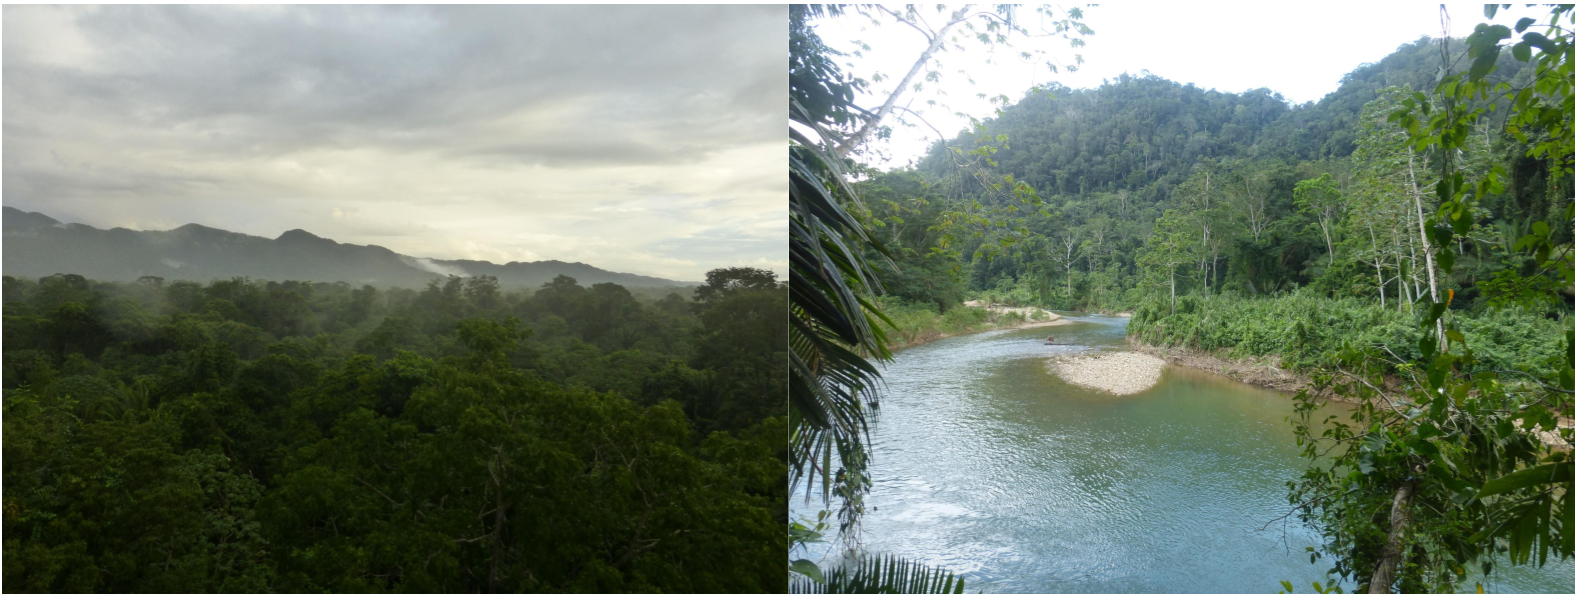
\includegraphics[width=0.9\textwidth]{Figures/TripPhotos.png}
\caption{Photos taken during the expedition to the Bladen National Reserve}
\label{fig:TripPhotos}
\end{figure}

\section{Study Sites}

We collected aerial survey data over two adjacent protected areas located in the Maya Mountains in the Toledo District of southern Belize ~\ref{fig:BFREE-Map}. The first was a 467-hectare (1,153-acre) private protected reserve administered by the Belize Foundation for Research and Environmental Education (BFREE; 16.5 N, 88.6 W).  The second site was a 170-hectare (420-acre) valley within the 39,270-hectare (97,039-acre) Bladen Nature Reserve (BNR), a national park-like, government reserve (Forestry Department, Government of Belize).  The two sites are part of the 607,028 hectares (1.5 million acres) Maya Mountains protected area system, often considered one of the largest remaining unspoiled, mixed tropical forest ecosystems remaining in Central America \cite{Brewer}, \cite{Olivet}, \cite{Dourson}.  Elevation and precipitation in the Maya Mountains range from 80 to 1000 meters with rainfall averages between 2500 and 3000 millimeters (80-100 inches) of rain per year. The area has distinct wet and dry seasons, of which $89\%$ of the rainfall occurs between May and December \cite{Brokaw}.  Both the BFREE and BNR areas have been classified with only coarse-scale, generalized habitat categories including: mainly tall and low tropical evergreen forest (low forest is referred to as “Broken Ridge” in Belize), and a variety of disturbed habitats including early secondary forest, riparian edge, seasonally inundated forests, and Cacao agroforest at BFREE; and tall to medium, tropical evergreen forests as well as smaller amounts of mixed low forest with some disturbed riparian edge near the Bladen River for the BNR.

For this we work we split these areas into three separate entities. First is BFREE area discussed above. Second is Oro which is a smaller valley that required to fly past BFREE along a river. Third is Ramos which required flying a considerable distance along a river before reaching a small open valley.

\begin{figure}[ht]
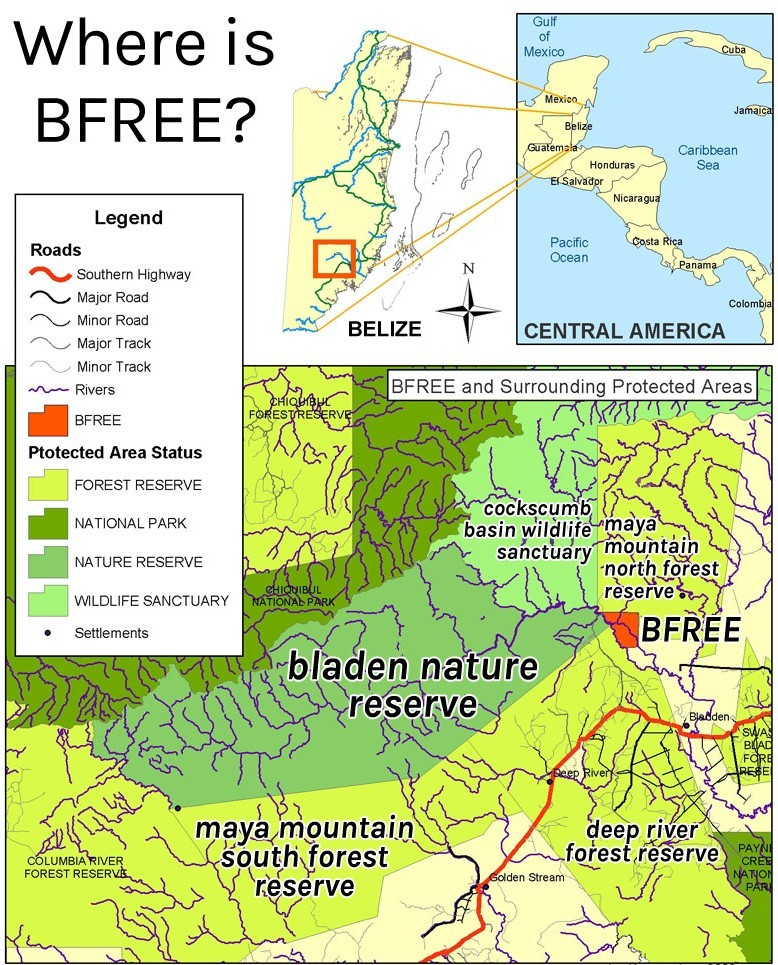
\includegraphics[width=0.4\textwidth]{Figures/BFREE-Map.jpg}
\caption{Map of Bladen Nature Reserve and BFREE site}
\label{fig:BFREE-Map}
\end{figure}

\section{Flight System}

The imagery was collected using a 2-meter wingspan, fixed-wing airplane-type UAV, model Volantex Ranger EX  ~\ref{fig:Volantex}. The Ranger was fitted with an Ardupilot autopilot system, which allows for autonomous control over long range flights. This flight system (Ranger + Ardupilot) was selected due to its rugged design, payload capacity, and long range. The tough body and 60 km range were requirements for use in Belize where landing areas were rough on the airframe. Flight paths were pre-planned in QGround Control Station, an open source ground control station software. All flights were conducted with a Sony QX1 for visible imagery, and a modified Canon S100 for near infrared, which limited vehicle range due to weight, but lowered the number of required flights. The cameras were triggered externally by the autopilot system based on distance flown. A bill of materials is given in table ~\ref{table:FlightBOM}. Collecting the same data using a manned flight system would be orders of magnitude more expensive.


\begin{table}[]
\centering
\caption{My caption}\label{table:FlightBOM}
\label{my-label}
\begin{tabular}{ll}
Item                                                    & Cost                          \\ \hline
ranger airframe                   & \$140.00 \\
ranger servos                     & \$150.00 \\
ranger power system (esc + motor) & \$150.00 \\
ranger telemetry kit              & \$200.00 \\
ranger rc                                               & \$40.00                       \\
3dr pixhawk                                             & \$200.00                      \\
pixhawk airspeed                                        & \$55.00                       \\
pixhawk gps/compass                                     & \$80.00                       \\
frsky taranis rc tx                                     & \$240.00                      \\
batteries                                               & \$500.00                      \\
gcs laptop                                              & \$200.00                      \\
chargers                                                & \$280.00                      \\
Sony QX1 + 20mm lens                                    & \$750.00                      \\
NGB Converted Canon S100                                & \$600.00                      \\ \hline
Total                                                   & \$3585
\end{tabular}
\end{table}

\begin{figure}[ht]
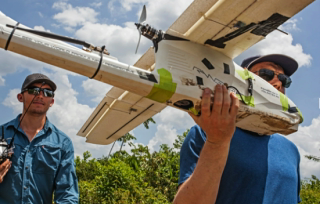
\includegraphics[width=0.6\textwidth]{Figures/Volantex.png}
\caption{Volantex Ranger Ex about to be hand launched for its last day of data collection. The platform is easily managed by a team of two people and can be launched without out external equipment making it an ideal platform for difficult to access areas.}
\label{fig:Volantex}
\end{figure}

\section{Flights}

Data was collected over three days over a total of six flights. The paths of all flights are shown in ~\ref{fig:FlightPaths}. All flights began from the same location on a dirt road in a corn field adjacent to the rainforest allowing for ample room for takeoff and landing. One of the downsides to commercial MAVs is that generally speaking they are not water proof nor very water resistant. Rainforests often have unpredictable weather patterns that interfere with flights. During this trip we were forced to cut several flights shorter than we desired.

\begin{figure}[ht]
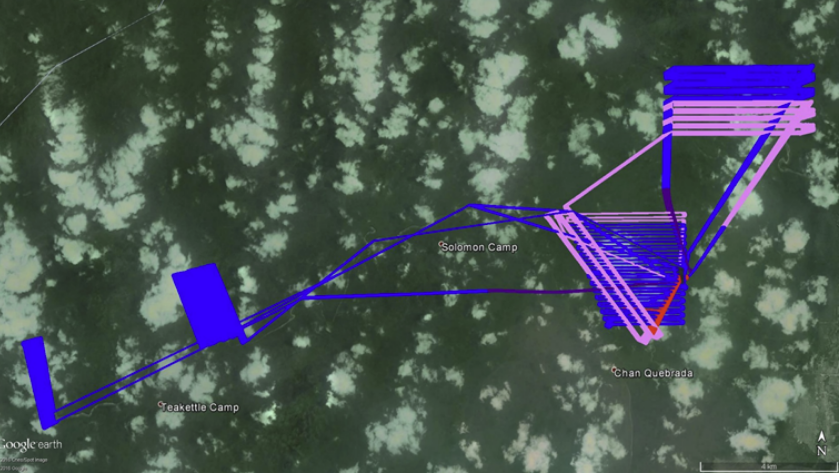
\includegraphics[width=0.8\textwidth]{Figures/FlightPaths.png}
\caption{Flight Paths Over BFREE, Oro and Ramos Survey Sites}
\label{fig:FlightPaths}
\end{figure}

\section{Post Processing}

\begin{figure}[ht]
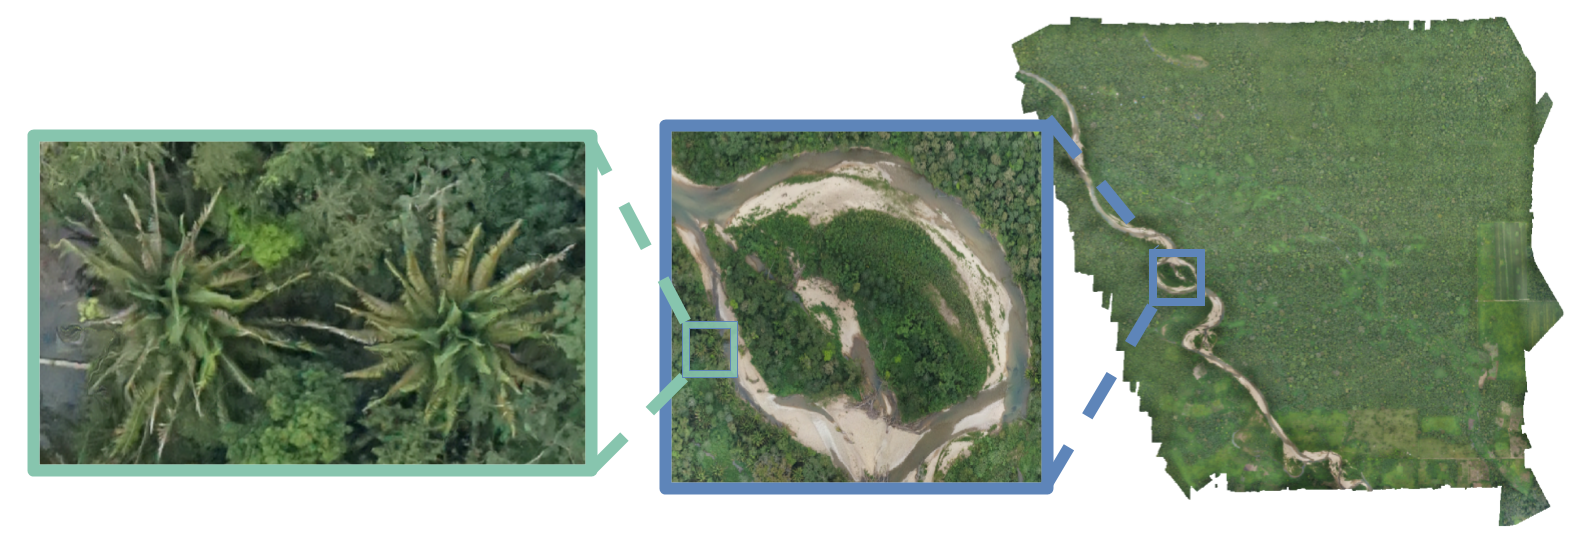
\includegraphics[width=0.8\textwidth]{Figures/Orthomosaic.png}
\caption{Orthomosaic of our main test site BFREE. An example of zooming down on the two palm trees is shown to demonstrate the resolution of the orthomosaic. The size of the orthomosaic is 16GB.}
\label{fig:Orthomosaic}
\end{figure}

The flight paths were designed to collect enough overlapping images to recreate the canopy in 3D and generate orthorectified mosaics through the process of SfM using Agisoft Photoscan Professional version 1.2.6. We produced three separate TIFs for the area: a RGB orthomosaic, a NIR orthomosaic, and a digital elevation map (DEM). The BFREE main survey site is a wide open with very little terrain. The lack of elevation changes allowed the UAV to safely fly at lower altitudes and collect higher resolution data. The resolution for the BFREE site is 4.93 cm/pixel covering a $8.73km^2$ site. The other two sites: Ramos and Oro lay along a river that cut through mountainous terrain which forced the UAV to fly at higher altitudes to maintain a safe boundary. The Ramos and Oro flights have nearly half the resolution with at around 10 cm/pixel with $20.50km^2$ and $16.37km^2$ respectively. Additionally these two flights encountered more low hanging fog and poor lighting conditions as can be seen in ~\ref{fig:OroClouds} making the task of classification more difficult. This requires the tree detector to be robust to resolution variations as well as lighting conditions.

\begin{center}
    \begin{table}[h]\footnotesize
        \caption{Post Processing Statistics generated by creating othrorectified mosaics through Agisoft.}\label{table:AgisoftStats}
        \begin{tabular}{| l | l | l | l | l |}
        \hline
        Site & Flying Altitude (m) & Number of Images & Resolution (cm/pixel) & Area ($km^2$) \\ \hline
        BFREE & 248 & 1529 & 4.93 & 8.73 \\
        Oro Main & 535 & 325 & 10.5 & 3.3 \\
        Oro Joiner & 543 & 156 & 10.5 & 2.27 \\
        Oro Path & 594 & 412 & 11.7 & 10.8 \\
        Ramos & 537 & 769 & 10.6 & 20.5 \\
        \hline
        \end{tabular}
    \end{table}
\end{center}

Additionally we used the Agisoft softare to generate orthorectified mosaics. Orthomosaics are similar to the panoramas popular on mobile phone; the basic premise being that by taking and stitching together many images you end up with a single cohesive image that represents an area larger than you could normally capture with a single photograph. Orthomosaics go a step farther by reprojecting the image into a top down view which is called orthorectification. See ~\ref{fig:Orthomosaic} to see the orthorectified image of the BFREE site. This is crucial to obtaining accurate population counts, since at most you want a single instance of a tree to be represented in the data. If we had simply used the raw images we might have had several pictures of the same tree.

Meta-data for each image i.e. GPS location and orientation is captured from the autopilot. This information allows the software to create a correspondence between each pixel in the orthomosaic and a global latitude, longitude. Meaning for each instance of a tree we find we can relate exactly where in the world that tree is located.

\begin{figure}[ht]
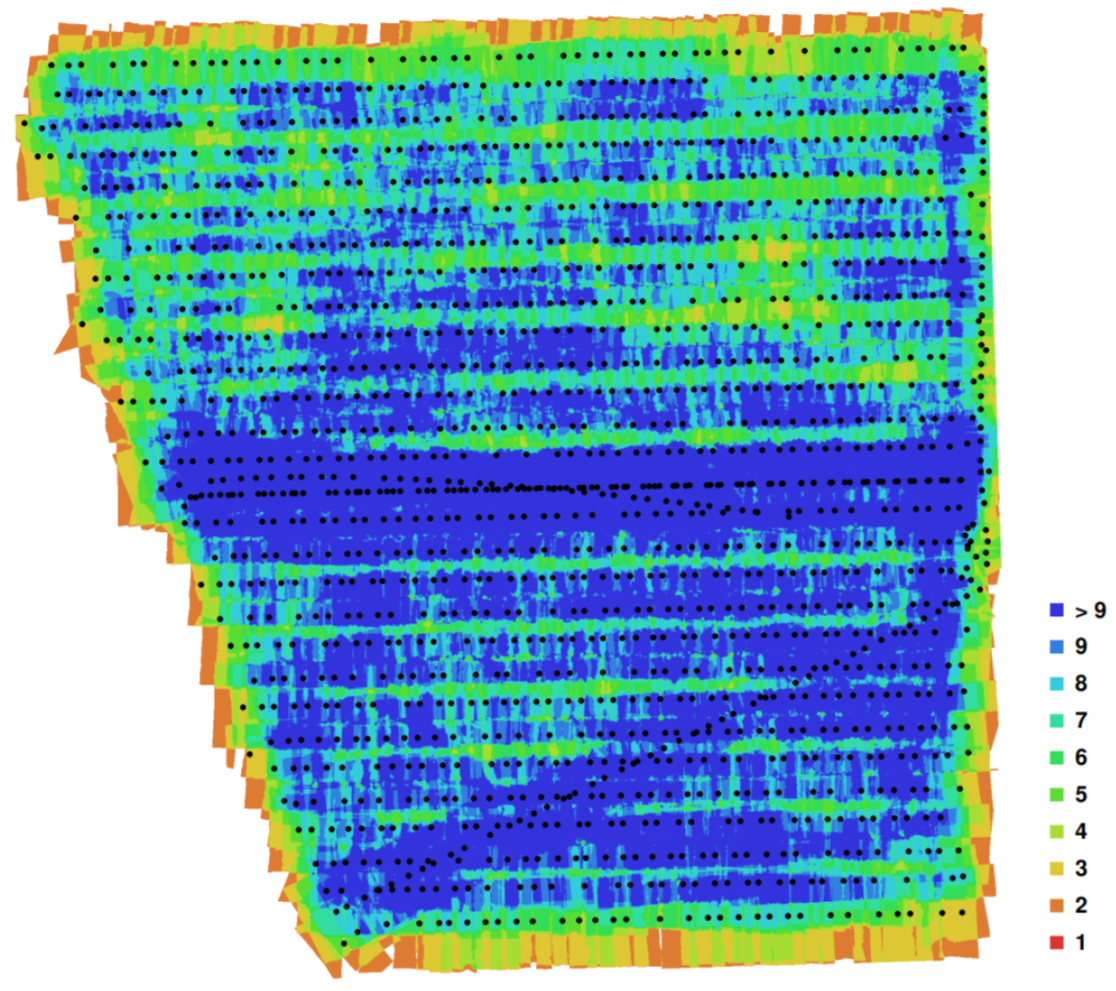
\includegraphics[width=0.8\textwidth]{Figures/BFREE-DEM.png}
\caption{Digital elevation map produced using Agisoft SfM software suite. Color codes represent the number overlapping images for that pixel. This additionally information could be very informative in discriminating between trees. Future research might examine how this information could be included in a CNN architecture.}
\label{fig:BFEE-DEM}
\end{figure}

\begin{figure}[ht]
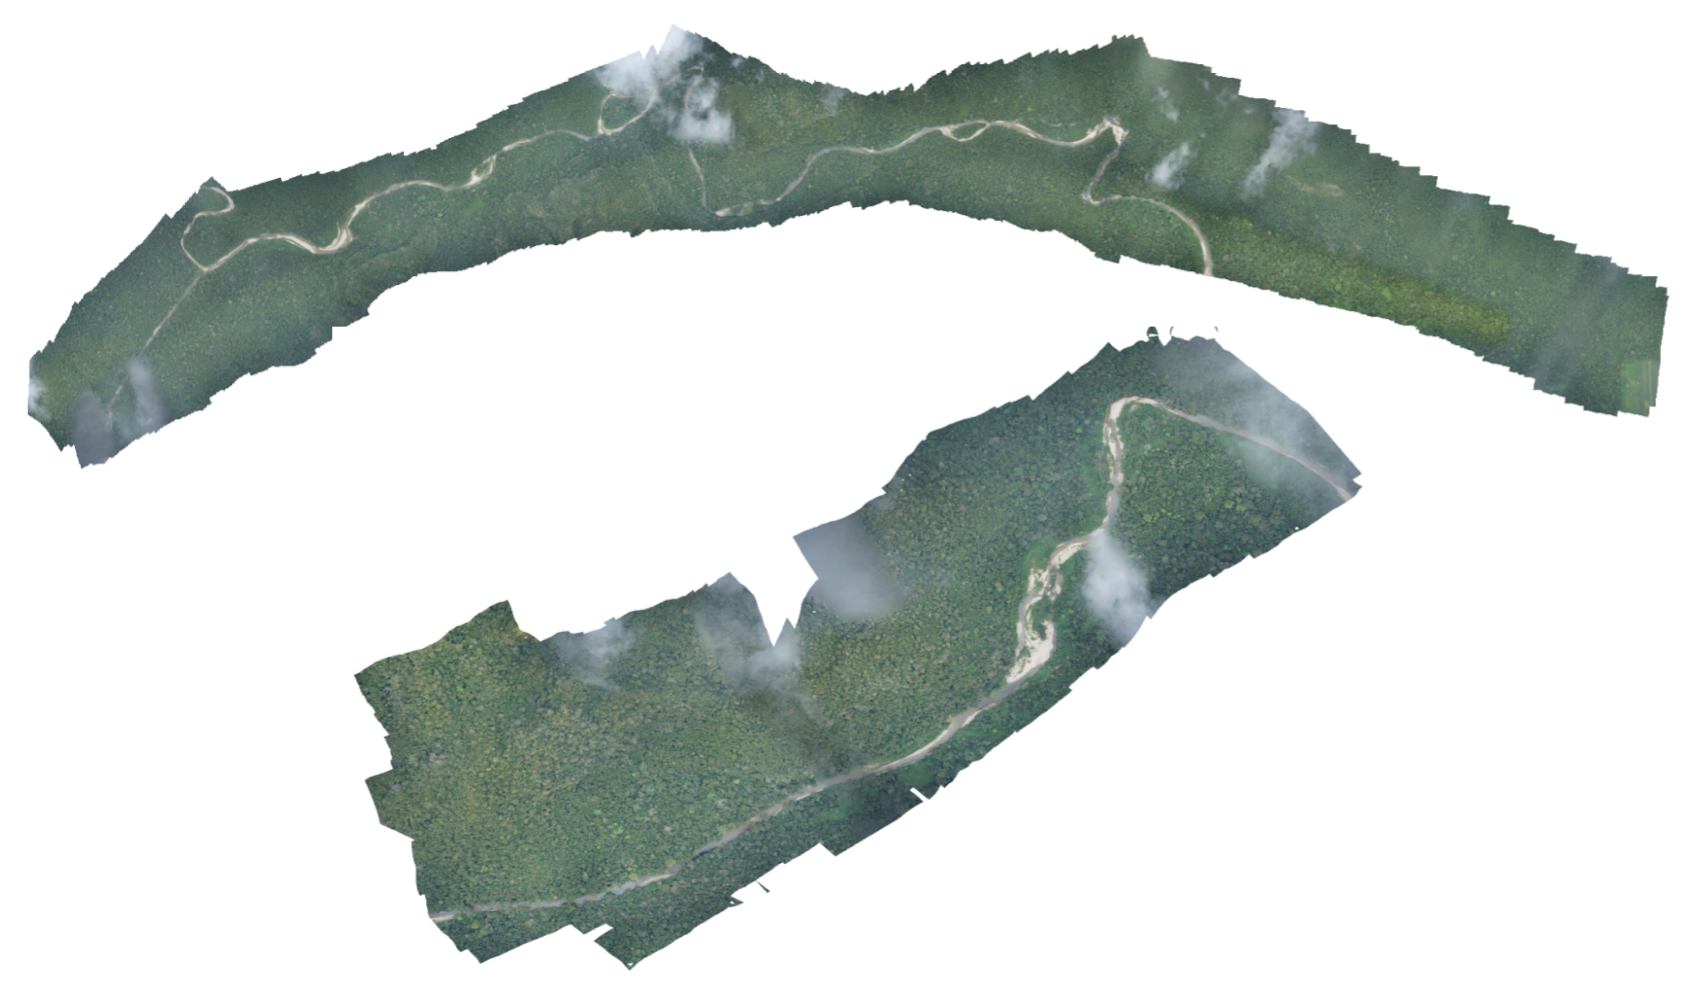
\includegraphics[width=0.8\textwidth]{Figures/OroClouds.png}
\caption{Two separate parts of the Oro site showing low hanging cloud coverage and various lighting conditions.}
\label{fig:OroClouds}
\end{figure}

% Chapter 4

\chapter{Applying Convolutional Neural Networks} % Main chapter title

\label{Chapter4}

%-------------------------------------------------------------------------------
%-------------------------------------------------------------------------------

\section{Creating the Dataset}

Creating an annotated dataset is often the longest and most tedious part of any machine learning task. A common complaint against deep learning is that you need large amounts of data to train properly generalized model. This can be mitigated somewhat through transfer learning, but for good generalization of a network sufficient training data is needed. The goal for our network is that it will be effective on other areas outside our main site of BFREE which might have variations in lighting conditions, pixel resolution, etc.. Our dataset can be found at DATASET-URL-INSERT-HERE.

\begin{figure}[ht]
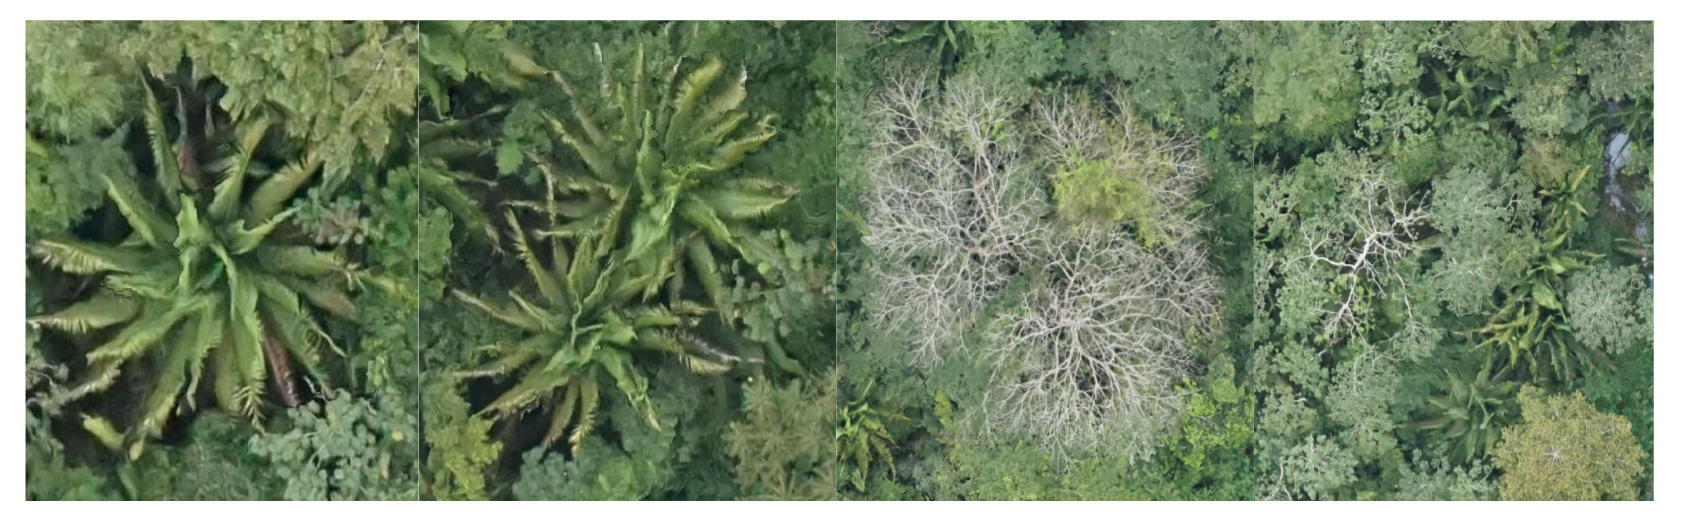
\includegraphics[width=1.0\textwidth]{Figures/Palm-Deciduous.png}
\caption{Example Instances of Cohune Palm Trees and Deciduous Trees from our dataset.}
\label{fig:Palm-Deciduous}
\end{figure}

\subsection{Labeling Tool}

In order to parallelize the labeling process we developed a simple web tool for decentralizing the task of labeling images. The web tool was a built using a mix of javascript and python; django was used to run the server and store data, openstreetmap was used for displaying the image and drawing boxes, and leaflet for working with GIS data. The web tool was run on a local server that allowed users to log on remotely and label data at their convenience. ~\ref{fig:LabelingTool} shows an example of using the tool. Users were given tiles cropped from the orthomosaic. Each tile corresponds to approximately $100m^2$ of rainforest. In order to help keep the labeling consistent a demo video was shown to volunteers that described how to label a tile. Each tile annotation contains a list of bounding boxes with a corresponding class label; either Cohune palm or deciduous. The data was stored on the server in a database and served as a CSV on request.

\begin{figure}[ht]
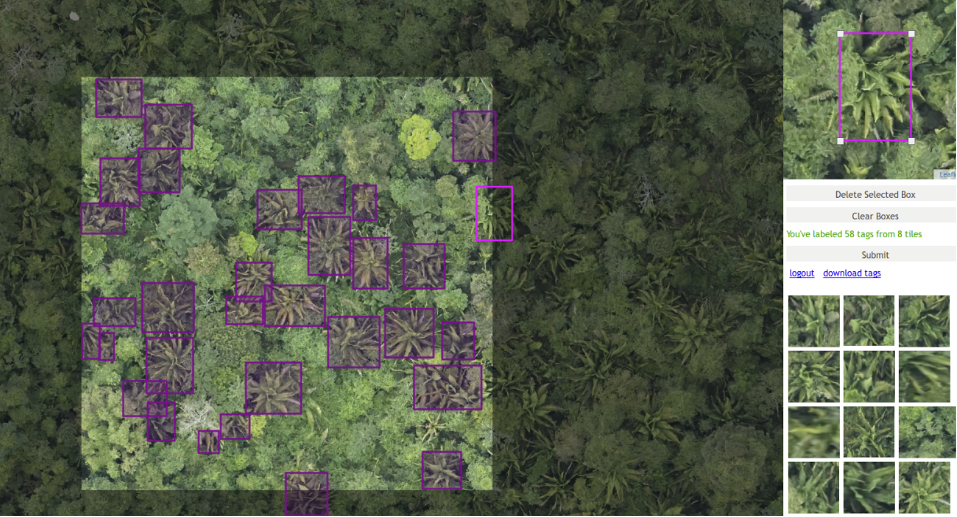
\includegraphics[width=1.0\textwidth]{Figures/LabelingTool.png}
\caption{Labeling tool in action. Note that you are shown surrounding area of the tile allowing the user to label palm trees that overlap two segments. Thumbnails on the lower right allow easy visual grepping of currently labeled trees}
\label{fig:LabelingTool}
\end{figure}

\subsection{Labeling Noise}

Our volunteers came from a mix of ecology students at the University of North Carolina Wilmington who labeled Cohune Palm trees and computer science students at University of California San Diego who labeled Deciduous Trees. Between labelers we found considerable variation in accuracy and annotation styles.

First we noticed that many tiles had obviously missing bounding boxes. We hypothesize that this is due to labeler fatigue. The tiles we present are quite dense with trees and are a very uniform green. The author noticed in his own labeling that over time it became harder to focus and be consistent with labeling. This could be mitigated in the future by presenting smaller tiles and limiting the amount of time users are allowed to label at one time.

Secondly we saw that bounding boxes with respect to crowding i.e. overlapping trees as well as occluded trees had a large variation. Some users created one box per crowd while some were meticulous in labeling each tree. Some users labeled tiny portions of heavily occluded palm trees while others skipped even partially occluded trees. One thought for future work would be to present users with examples for each scenario and then present tests which are used to evaluate the labelers skill.

In order to combat this label noise the author went through the dataset and cleaned up bounding boxes with respect to crowded or occluded trees and added missing annotation to each tile. This led to significantly lower average loss and higher evaluation metrics.

\subsection{Dataset Statistics} \label{section:statistics}

In order to get a better understanding of the dataset we examine the position of each bounding box in the image frame as well as the distribution of the square root of bounding boxes areas. The latter is very import as its informative for choosing bounding box priors for the network. Notice that the distribution for each class is roughly Gaussian centered around mean $210 pixels^2$ for Cohune Palms and $130 pixels^2$ for Deciduous trees. Deciduous trees by inspection have a much higher standard deviation then Cohune Palms with more outliers. Also note that we have a heavy class imbalance with approximately 10x Cohune Palm Trees when compared to Deciduous Trees. This will be addressed in ~\ref{section:class_imbalance}.

\begin{figure}[ht]
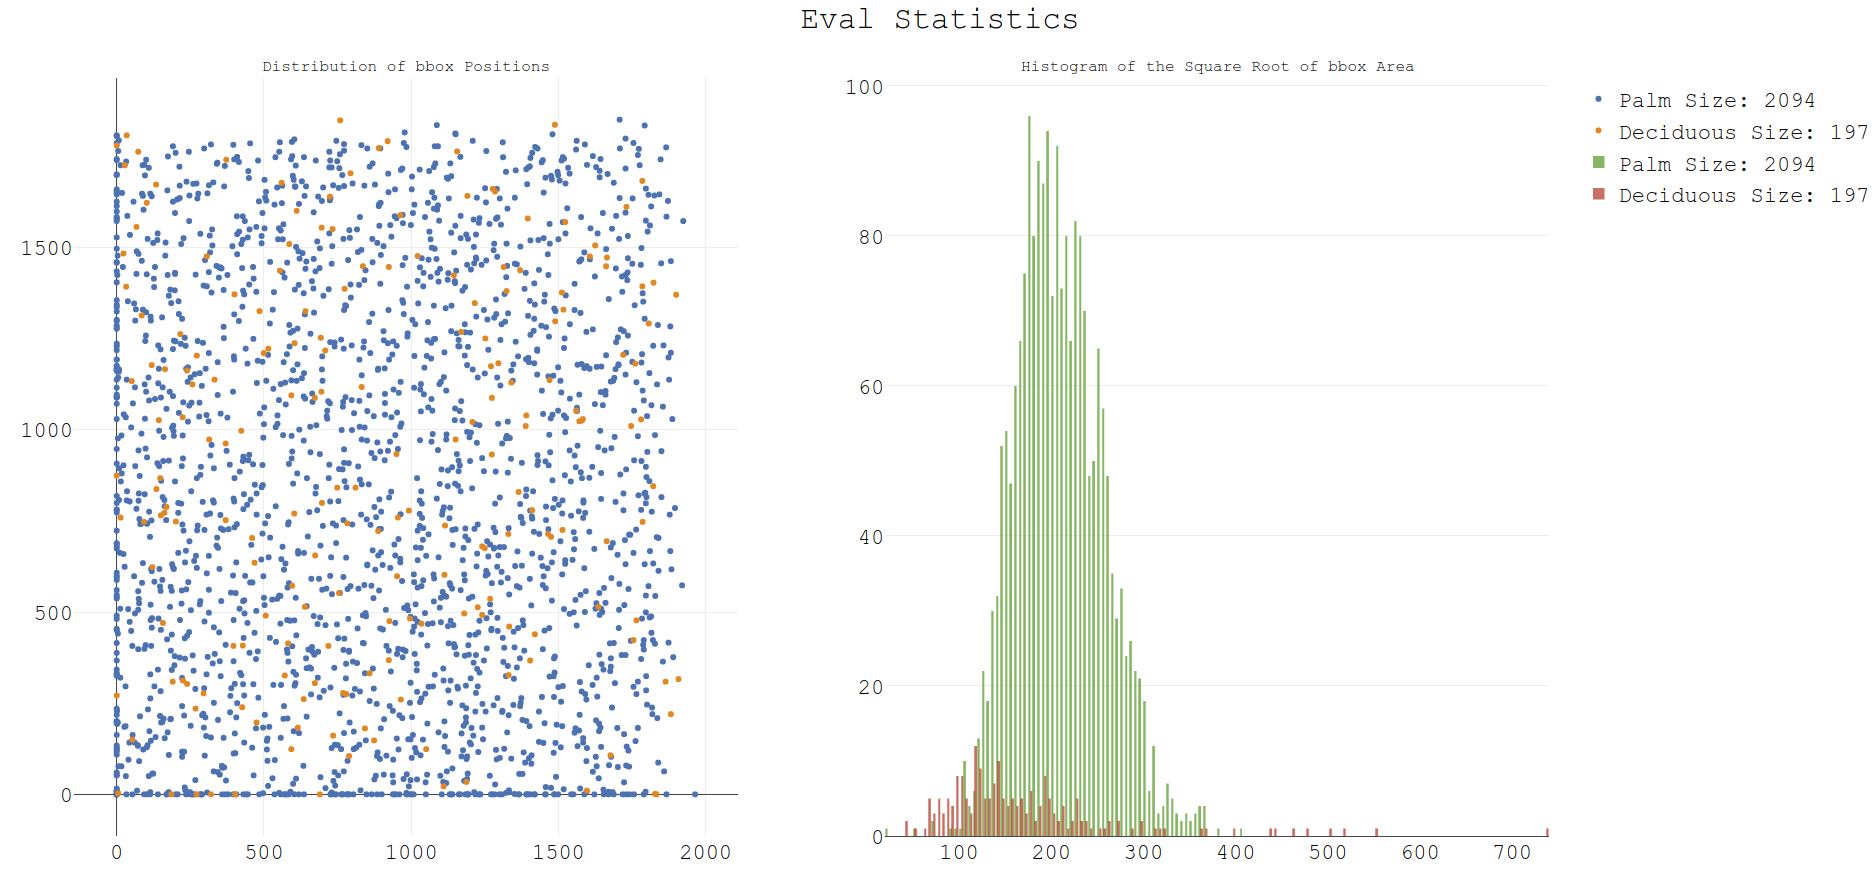
\includegraphics[width=1.0\textwidth]{Figures/EvalStats.png}
\caption{Bounding Box Statistics from the Evaluation set.}
\label{fig:EvalStats}
\end{figure}

\begin{figure}[ht]
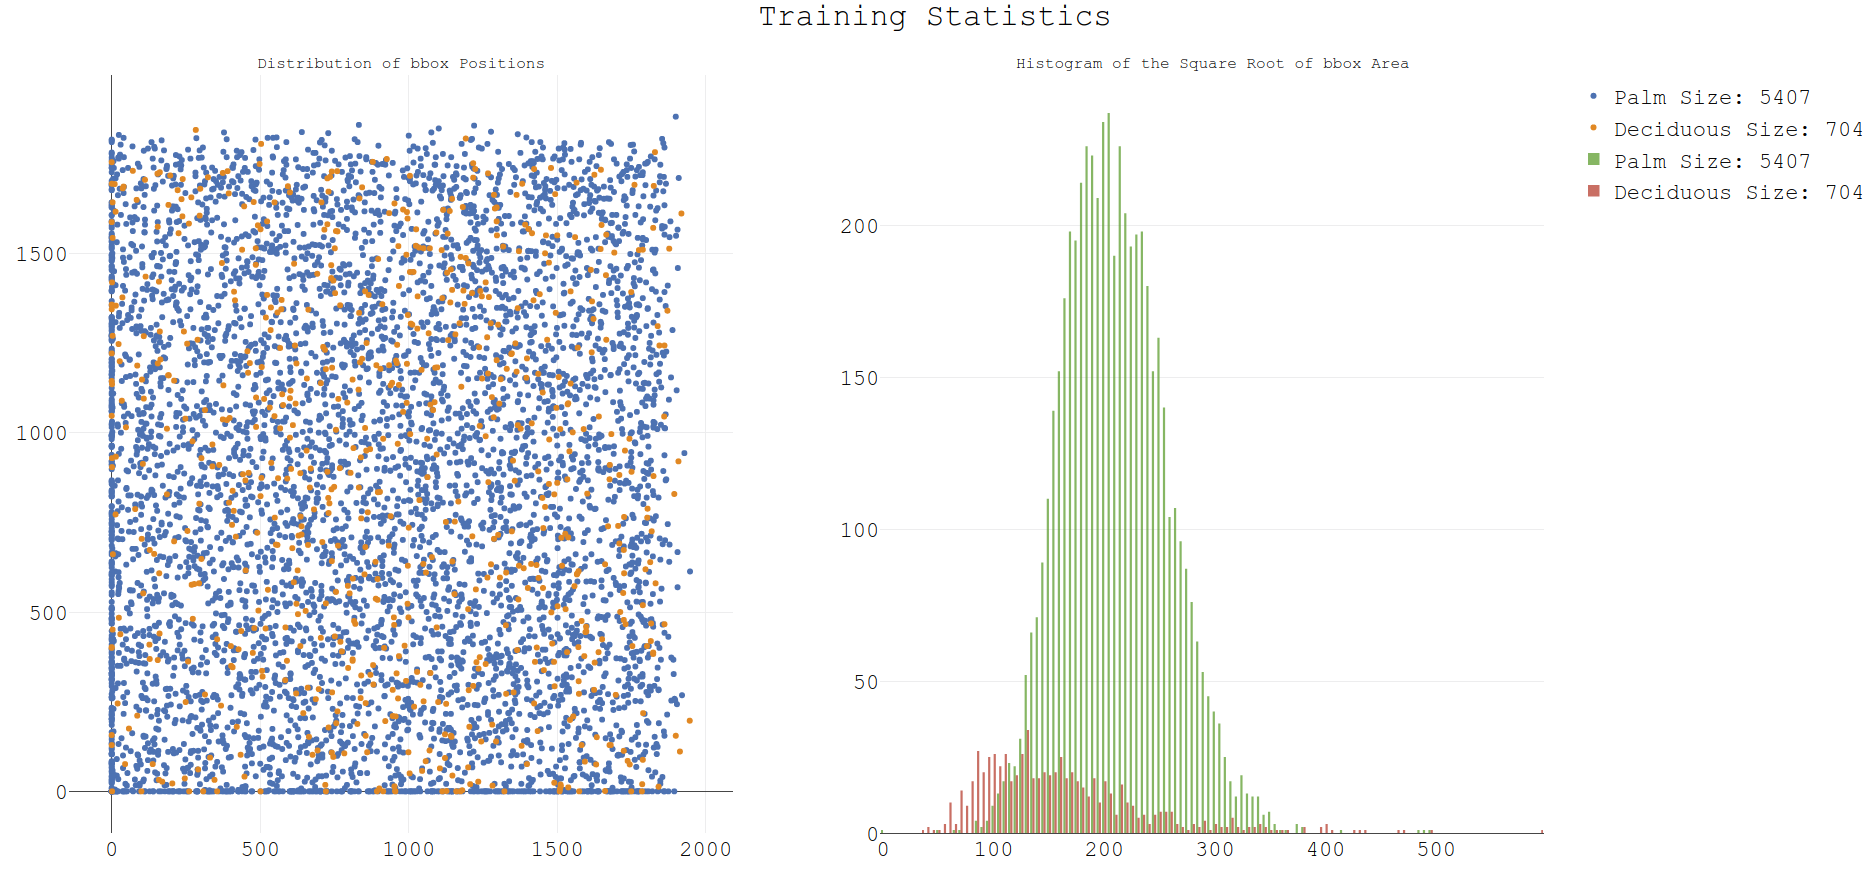
\includegraphics[width=1.0\textwidth]{Figures/TrainingStats.png}
\caption{Bounding Box Statistics from the Training set.}
\label{fig:TrainingStats}
\end{figure}

\section{Training the Network}

The dataset we present is still relatively small compared to many used to train deep neural networks from scratch. We compensate by using a pretrained network. YOLOv2 comes with several pretrained networks on the common classification datasets ImageNet and object detection datasets COCO \cite{COCO}, Pascal VOC \cite{VOC}.

The main difference between the pretrained networks is that the ImageNet weights do not include the final convolution layer which is used for regression while the other two pretrained networks do. We found that training with the ImageNet base network led to better performance. We hypothesize that this is because the other networks have already over fit the regression task to the bounding box shapes and classes in the object detection datasets.

We trained our networks using NVIDIA GTX 1080 graphics card, Intel Core i7 7th gen, and 32GB of RAM. The full desktop setup cost was under $\$3000$. On average we trained for approximately 20,000 iterations on our dataset with a batch size of 32 taking roughly 18 hours. We used a simple learning rate schedule that started at 0.001 and dropped by 10x every 7,500 iterations. This is a fairly short training regime when compared to training on a dataset which may contain upwards of a million images like ImageNet.

\begin{table}[]
\centering
\caption{My caption}\label{table:DesktopBOM}
\begin{tabular}{ll}
item                & cost       \\ \hline
Noctua NH-L12       & \$60.00    \\
NVIDIA GTX 1080     & \$700.00   \\
Silverstone ML07    & \$70.00    \\
Corsair SF 600W     & \$120.00   \\
Samsung 850 EVO 1TB & \$350.00   \\ \hline
Total               & \$1,970.00 \\
\end{tabular}
\end{table}


\subsection{Network Resolution}

YOLOv2 takes advantage of its ability to have dynamically resized inputs in training by randomly resizing the network input every 10 iterations. This has the effect of training on various resolutions of data making the algorithm more robust to variance in resolution at run time; an important step to generalizing our network to images with lower resolution. We limit the resize to three strides above and below our desired input resolution i.e. if our desired inference resolution is 416 then the lower limit on training would be 320 and the maximum would be 512. We experiment with three different resolutions, 416, 608, 800 and show the performance of each at ~\ref{section:results}.

\subsection{Class Imbalance}\label{section:class_imbalance}

Our dataset suffers from a large class imbalance between Cohune Palm Trees and Deciduous trees as shown in ~\ref{fig:TrainingStats}.

\section{Evaluating the Network}

Evaluating the performance of the network for an object detector is much less straight forward then for a classification network. We not only have to classify an object but we need to judge how well the generated bounding boxes match the ground truth; all the while trying to minimize the number of false positives that are produced. With the number of variables being juggled different interpretations arise for what a \textit{good} network performance looks like. A commonly accepted metric used by \cite{COCO} is Average Precision (AP) which is a single value that attempts to capture a coherent metric of precision. While others might display performance as the relationship between probability of detection vs probability of false alarm. In the next paragraph I will cover the basics of evaluating detections and the metrics we adopt for this work.

Detections generated by the network for an image fall into three categories: True Positive (TP), False Positive (FP), and False Negative (FN). In order to classify a detection as TP, FP, or FN we define Intersection over Union (IoU) between a network generated bounding box and a human bounding box as $IoU = \frac{Intersection of Boxes}{Overlap of Boxes}$. See ~\ref{fig:IOU} for an example of IoU. Given network detections and human labels for an image we can define TP as a network detection and human label with an IoU greater than a certain threshold and a matching class. Both the Pascal VOC and COCO datasets evaluate results using an IoU of $50\%$ and we adopt this standard. Furthermore there can only be a single TP per ground truth. If there are more than one network detection that meet the criteria for TP the detection with max IoU is accepted and the rest are considered as FPs. FPs are all network detections that do not have a corresponding ground truth. FN are all human labels that do not have a corresponding network detection. Now we can define $precision = \frac{TP}{TP+FP}$ and $recall = \frac{TP}{TP + FN}$ as the two metrics we will use to evaluate performance. Precision gives a sense of how relevant the returned detections are i.e. high precision corresponds to returning mainly good detections with few false positives. While recall represents the percentage of human labels correctly returned.

Each network detection has an associated confidence in how likely it thinks there is an object of that class present at that location. In order to calculate Average Precision we divide our confidence threshold from $0$ to $1$ with steps of size $0.01$. We then calculate precision at each step in our confidence range excluding any detection that have a confidence below that threshold which are then averaged to find AP. Another common way to represent network performance are precision recall graphs. We calculate recall at each confidence threshold like before and then simply plot the precision and recall as a pair. The desired shape for a PR curve is a knee which shows that precision remains high as recall increases and confidence threshold decreases.

We use pycoco api open source evaluation tools \cite{COCO} to keep our results consistent with state of the art object detection evaluation metrics. This also means our dataset is in the COCO format and can thus be trained on any open source object detector that uses that format for training and evaluation.

\begin{figure}[ht]
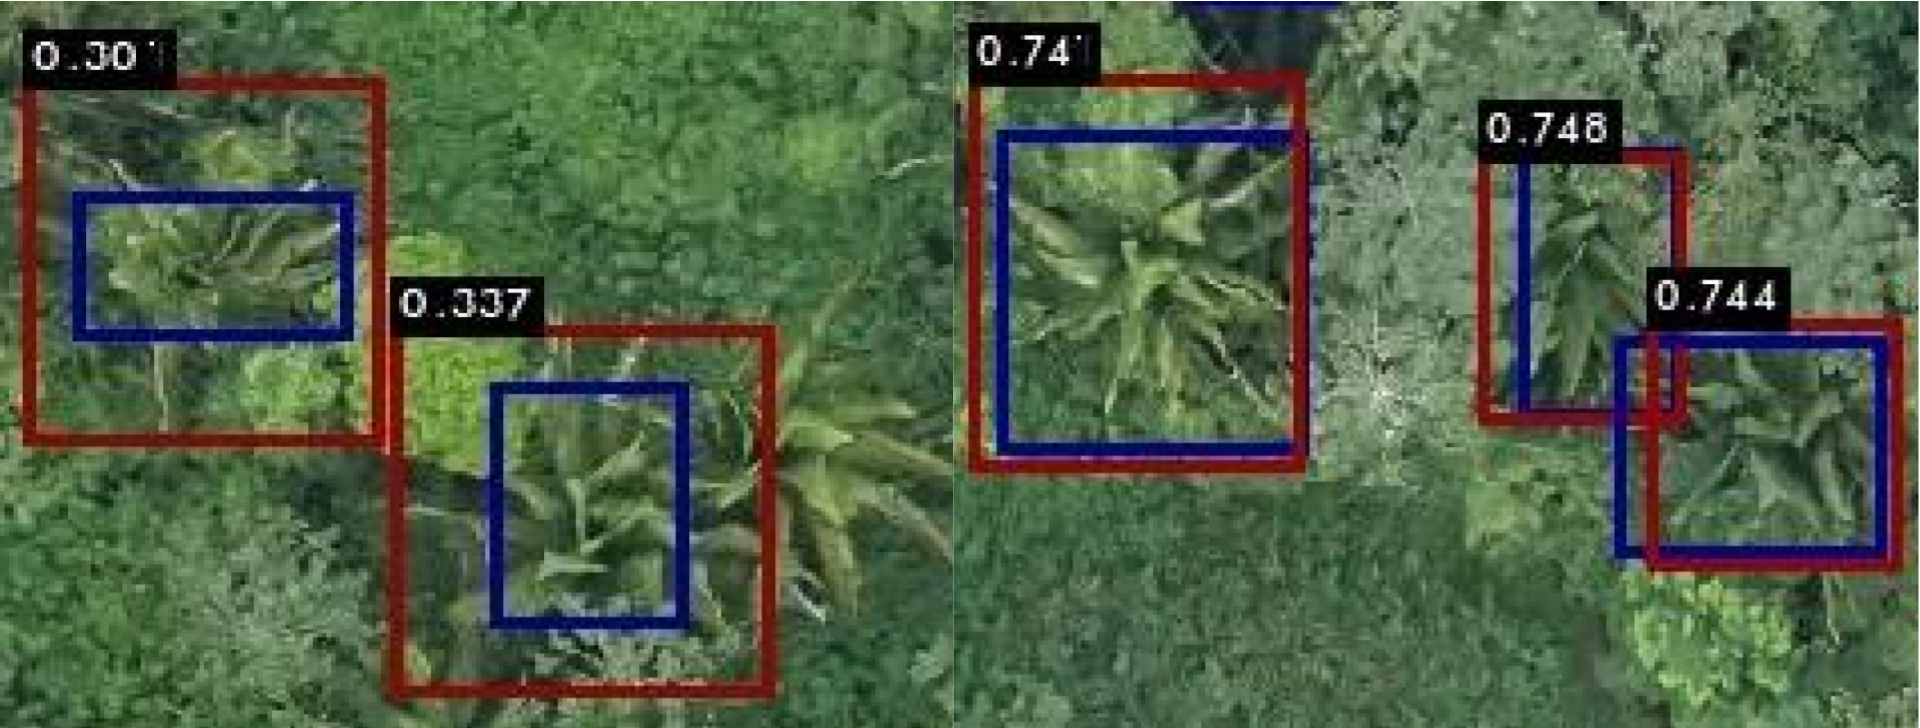
\includegraphics[width=1.0\textwidth]{Figures/IOU.png}
\caption{Example of IOU scores where blue corresponds to the human box and red corresponds to network detections.}
\label{fig:IOU}
\end{figure}

% Chapter 5

\chapter{Results} % Main chapter title

\label{Chapter5}

%-------------------------------------------------------------------------------
%-------------------------------------------------------------------------------

\section{Results}\label{section:results}

Preliminary results show distinct patterns in the distribution of both Cohune Palm and deciduous trees. Our best results using YOLOv2 CNN to classify the individual trees resulted in an average precision (AP) of $79.5\%$ for Cohune Palm and $67.3\%$ AP for deciduous trees ~\ref{fig:PR-palm-deciduous-bfree} at the main BFREE site. Furthermore testing at our more distant sites: Oro and Ramos we scored an $67.1\%$ and $76.0\%$ AP on Cohune Palms and $64.9\%$ and $84.2\%$ AP on Deciduous trees respectively. See table ~\ref{table:ap-results} below. This shows that our network was able to generalize enough to more distant sites that had both lower resolution and different lighting conditions due to low hanging clouds.

\begin{center}
    \begin{table}[h]\footnotesize
        \caption{Average Precision for each site per class}\label{table:ap-results}
        \begin{tabular}{| l | l | l | l |}
        \hline
        Site & Resolution (cm/pixel) & Cohune Palm (AP) & Deciduous Trees (AP)\\ \hline
        BFREE & 4.93  & $79.5\%$ & $67.3\%$ \\
        Oro   & 10.95 & $67.1\%$ & $64.9\%$ \\
        Ramos & 10.60 & $76.0\%$ & $84.2\%$ \\
        \hline
        \end{tabular}
    \end{table}
\end{center}

For both Oro and Ramos the size of evaluation set of spiny trees is very small due to scarcity of deciduous trees in the labeled areas. Examining the outlier of Ramos spiny results revealed that the area labeled had a high number of easy detections as well leading to better then average results.

\begin{figure}[ht]
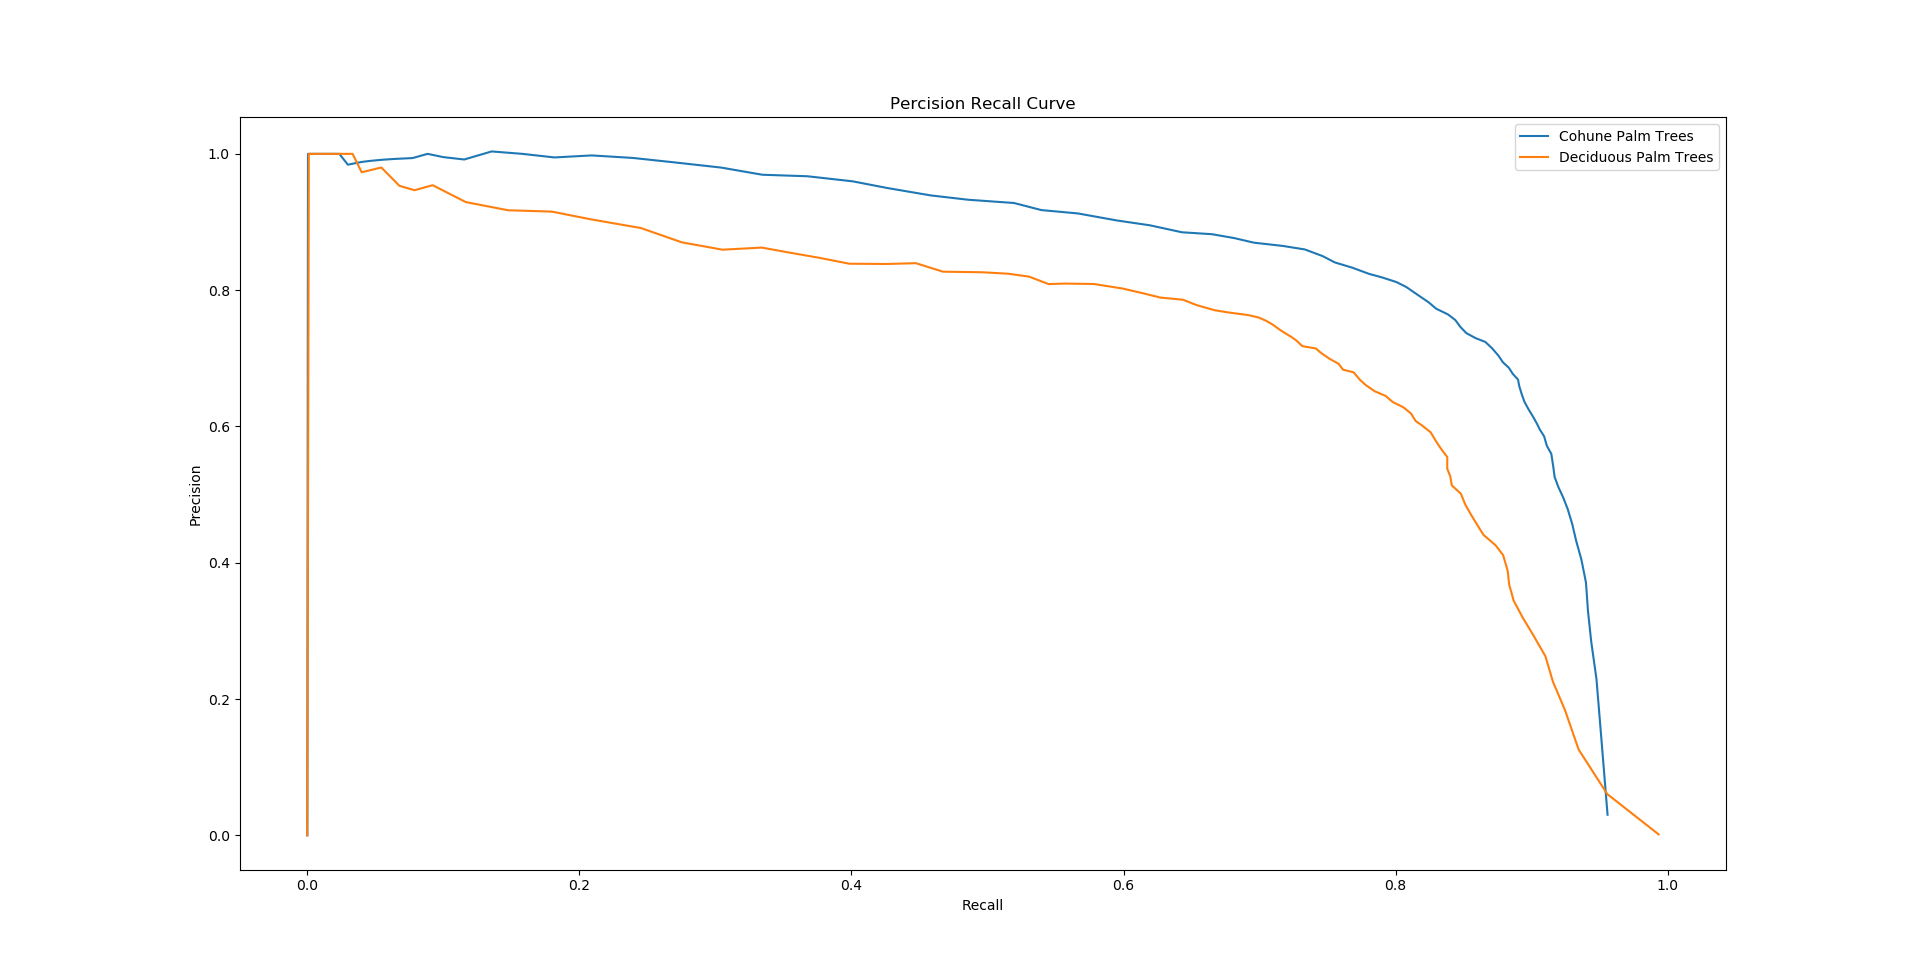
\includegraphics[width=1.0\textwidth]{Figures/PR-palm-deciduous-bfree.png}
\caption{Precision Recall for Cohune Palm Trees vs Deciduous Trees. We noticed a substantial intraclass difference with deciduous tree size and shape, correspondingly the network had a difficult time localizing individual trees with a high IOU.}
\label{fig:PR-palm-deciduous-bfree}
\end{figure}

\subsection{Effect of Network Resolution}

One aspect we explore in this work is the input resolution of the network. We found that it provided a mild boost of roughly $.8\%$ for our bfree site. However, it produced significantly better results for both Cohune Palm Trees and Deciduous trees of both Ramos and Oro. We hypthosize this is because the image resolution was already have of our main sites that any further down sampling to fit into the network input significantly hurt our performance.


\subsection{Effect of Image Resolution}

In ~\ref{fig:PR-resolution} we show the PR curves for various resolution of data starting for Cohune Palm trees starting from our base resolution of ~5 cm/pixel and going to 1m/pixel. The resolutions were artificially created by subsampling the original images as shown in Figure 11. Within the 5-20cm/pixel range we still have workable results; past 40 cm/pixel we seen a rapid decline. Typical satellite imagery lives in the range of 3 meters to 30 cm with the cost getting proportionally higher as resolution increases. We show with this technique that it is necessary to have very high resolution imagery in order to do fine grained species classification. More performance from the network might have been possible with greater tuning and training for lower resolution imagery; however, we believe that we are close to the upper limit. As the pictures in ~\ref{fig:Palm-resolution} show at a certain point the palm becomes indistinguishable to humans putting a bound on our ability to even create a dataset with which to train our network.

\begin{figure}[ht]
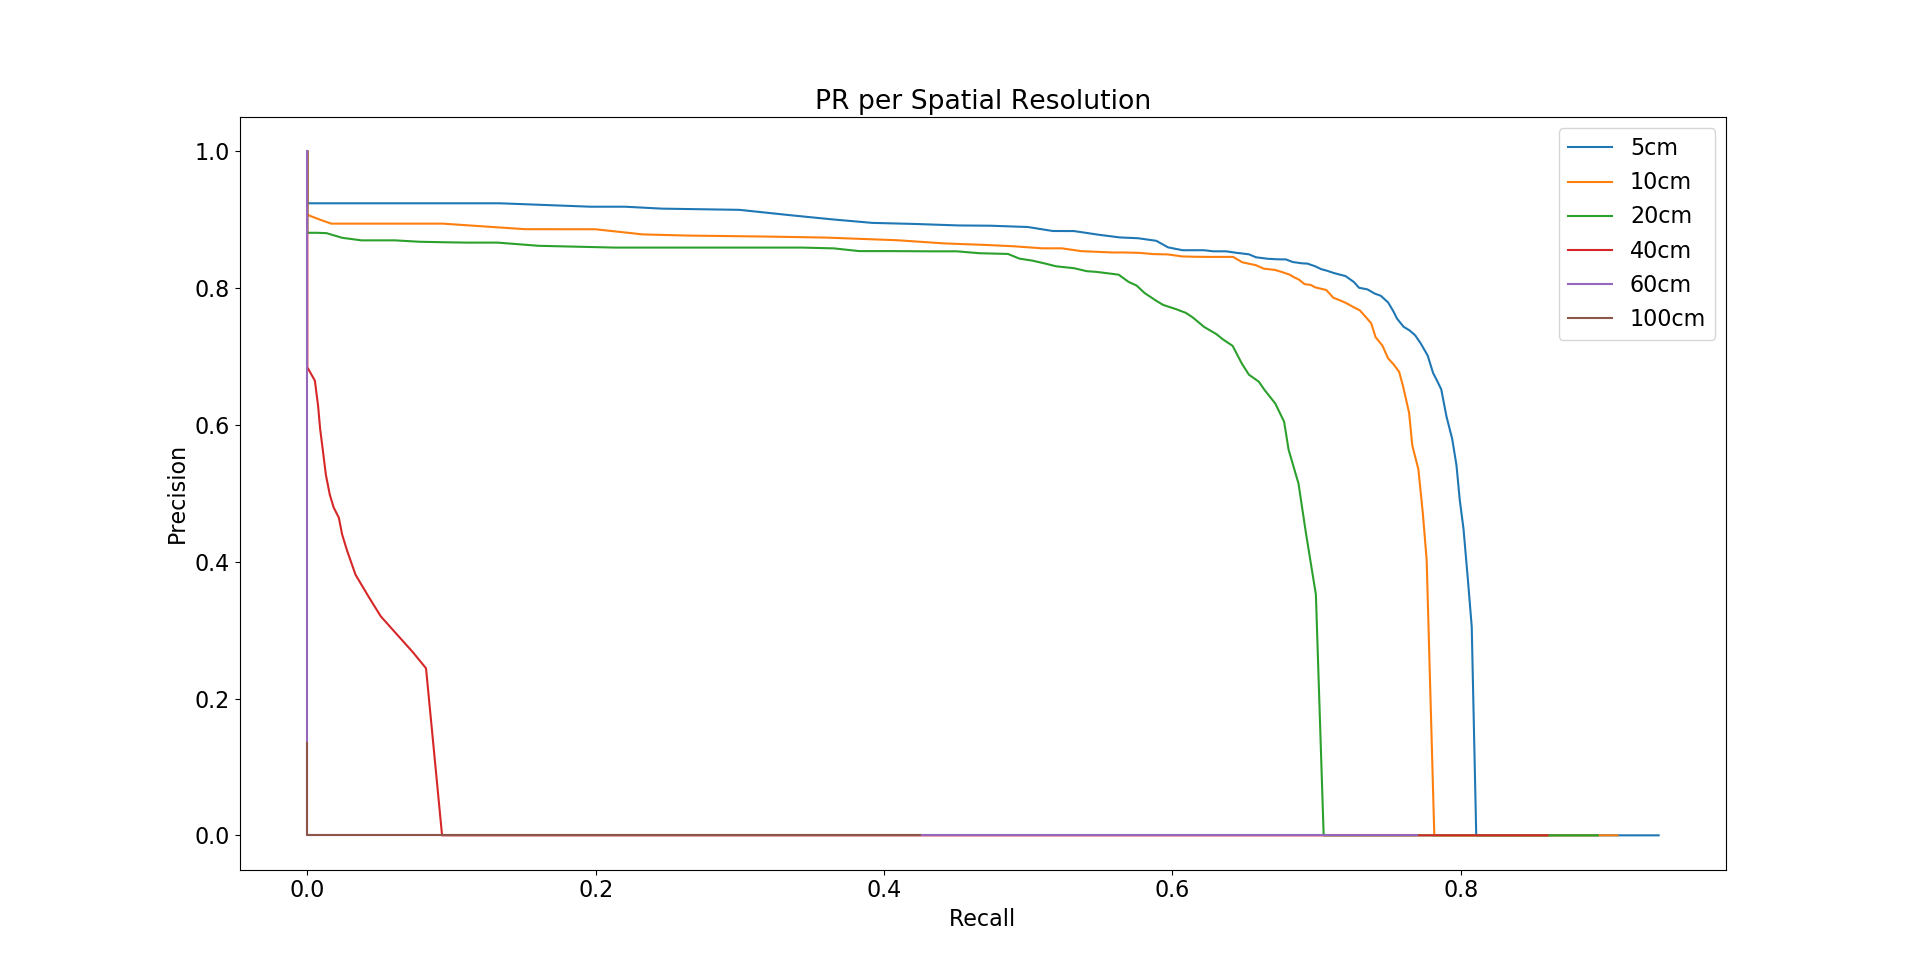
\includegraphics[width=1.0\textwidth]{Figures/PR-resolution.png}
\caption{Evaluating Precision Recall vs spatial resolution is important for planning future flights since gathering higher resolution requires flying at lower altitudes meaning you can cover less distance. Ideally we can find a sweet spot between image resolution and performance that lets us maximize area covered.}
\label{fig:PR-resolution}
\end{figure}

\begin{figure}[ht]
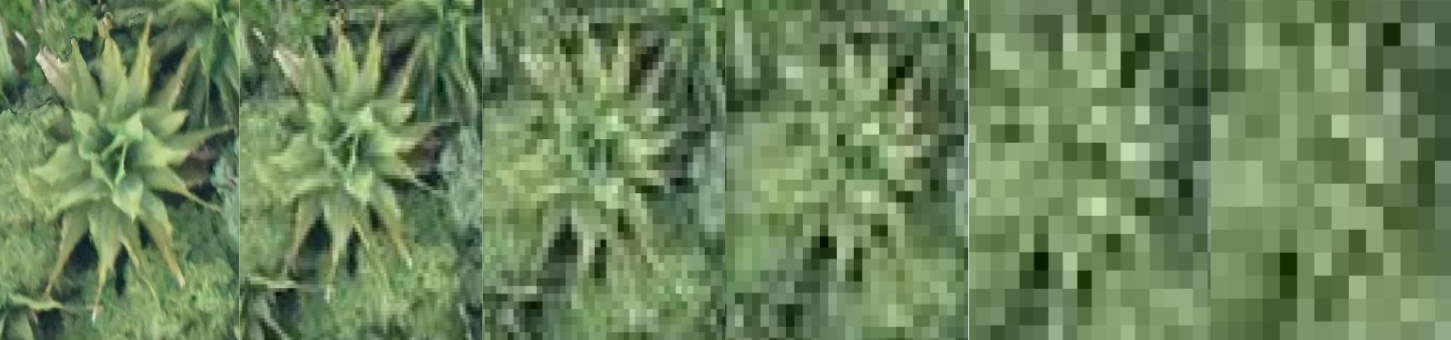
\includegraphics[width=1.0\textwidth]{Figures/Palm-resolution.png}
\caption{Resolution in cm/pixel from left to right: 5, 20, 40, 60, 80, 100. It is clear that after 60 cm/pixel the image becomes indiscernible.}
\label{fig:Palm-resolution}
\end{figure}

\subsection{Class Imbalance Issues}

Class imbalance played a large roll in our training. We found that training on both classes produced networks that could not localize deciduous trees at all. This is because the signal from Cohune Palm trees heavily out weights that of the deciduous trees during back-propagation. In the future we would like to explore weighting the loss function in order to place more emphasis on examples from classes with fewer instances.

\subsection{Ecological Impact}

We identified 6,308 palms at BFREE, yielding 120.4 ha palm coverage. Palms were more prevalent at BFREE, (disturbed) with $21\%$ palm cover, compared to only $5.9\%$ and $2.0\%$ in our less-disturbed, mountain sites (BNR). Total palm coverage in the BNR ranged from 6.2 ha - 27.3 ha. Our preliminary data for deciduous trees at BFREE resulted in identifying 2,389 trees with a total coverage of 17.8 ha or $3.0\%$. Our results conform well with past on-the-ground data for both tree types. Cohune palms tend to grow in disturbed areas, but also contribute to soil organics. Deciduous tree crown area calculated in comparable rainforests ranged from $~3-10\%$. This study shows how UAV and CNNs can save time (vs. manual) identifying specific tree species, helping to determine key rainforest habitat characteristics, as well as aid research and management of remote areas.

\begin{figure}[ht]
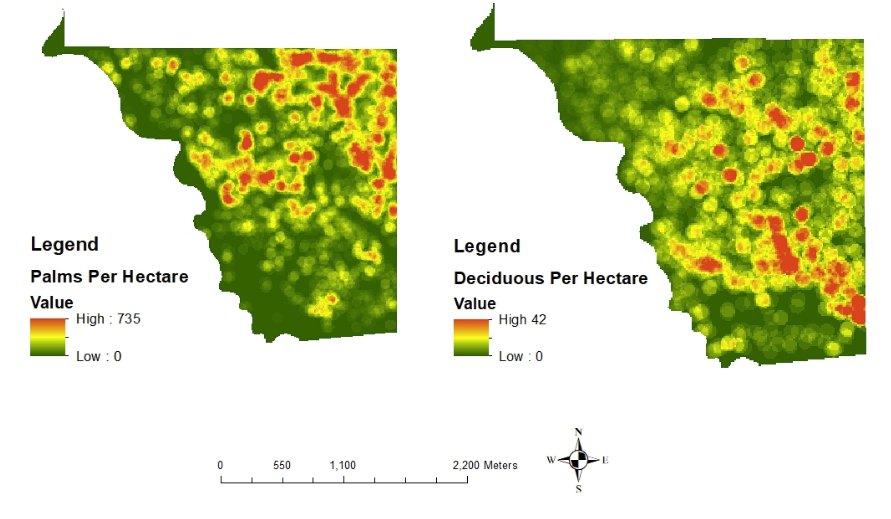
\includegraphics[width=1.0\textwidth]{Figures/HeatMaps.png}
\caption{Left: Cohune Palm Trees Right: Deciduous Trees. Note that the two classes of trees grow in distinct location from each other.}
\label{fig:HeatMaps}
\end{figure}

% Chapter 6

\chapter{Further Studies} % Main chapter title

\label{Chapter6}

%-------------------------------------------------------------------------------
%-------------------------------------------------------------------------------

\section{NOAA Dataset}


\begin{figure}[ht]
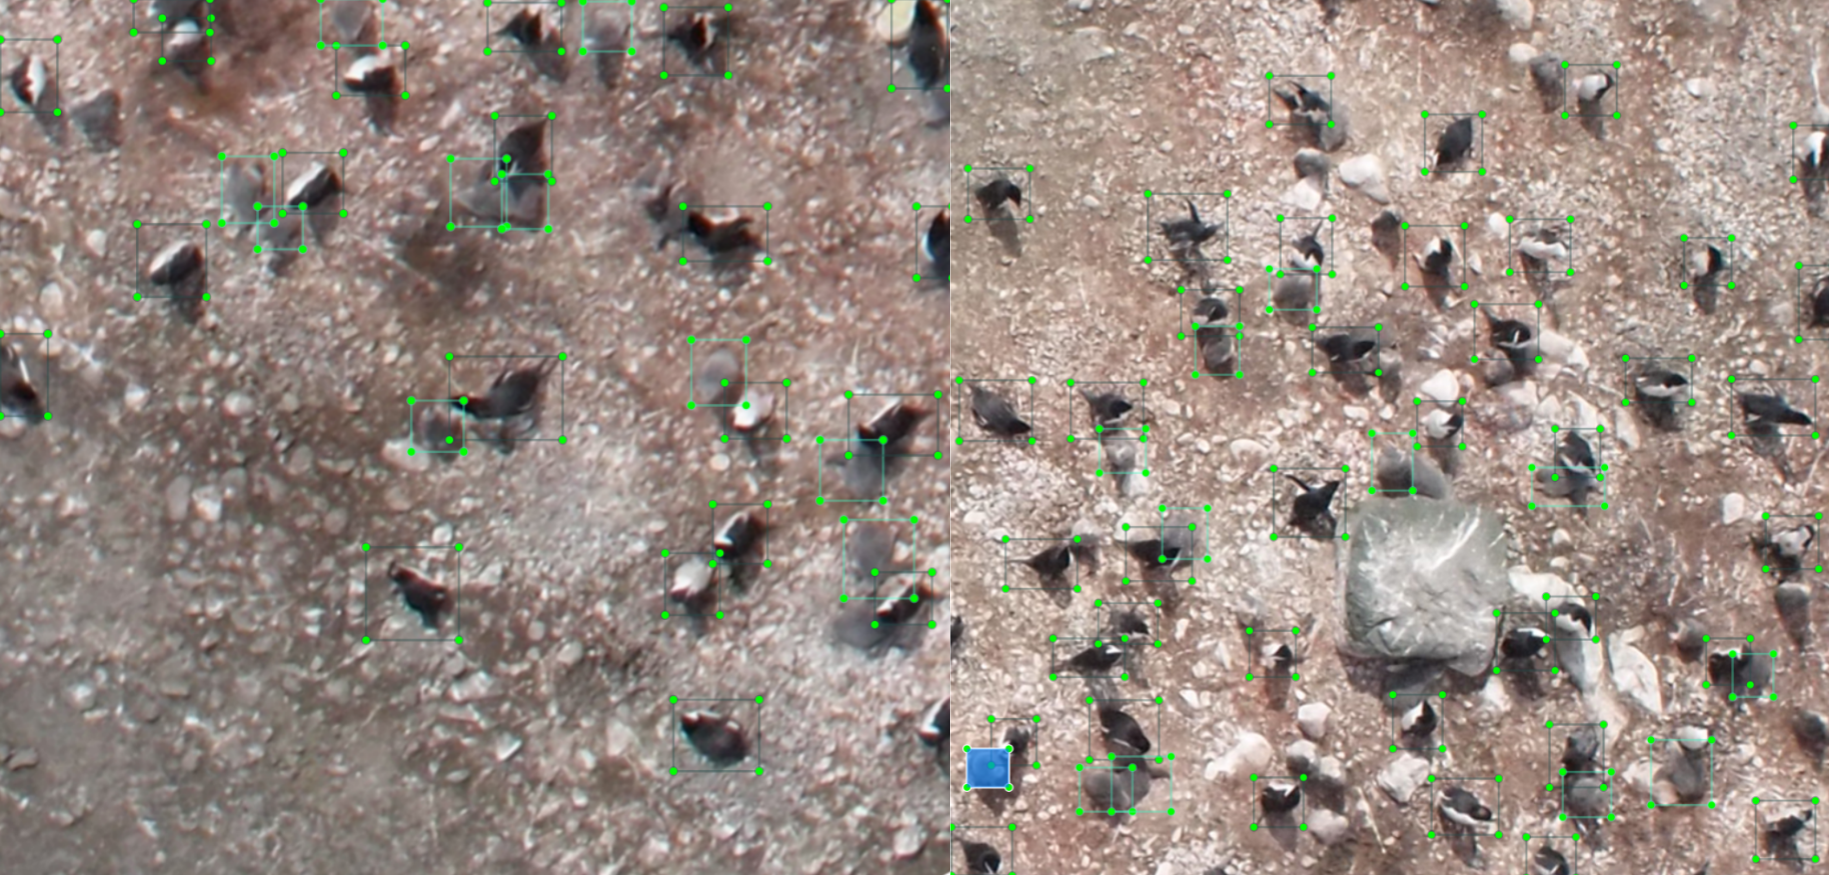
\includegraphics[width=1.0\textwidth]{Figures/Penguins.png}
\caption{}
\label{fig:Penguins}
\end{figure}

\begin{figure}[ht]
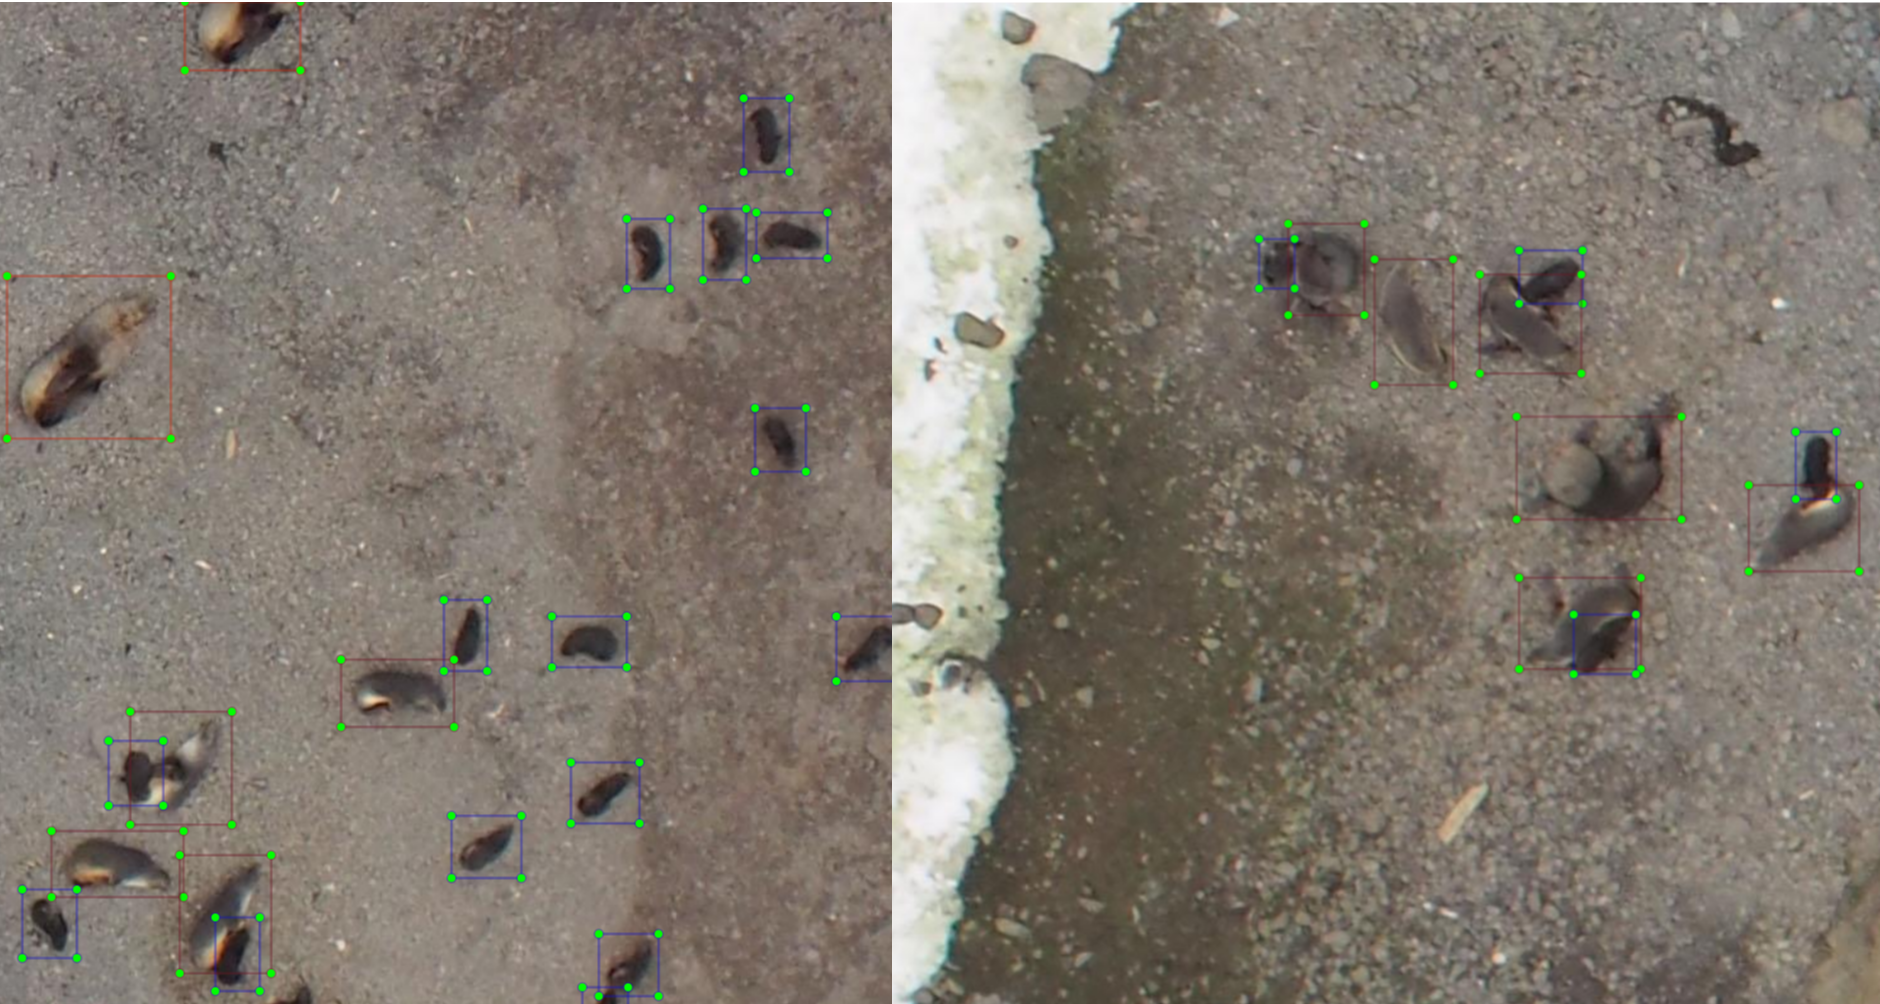
\includegraphics[width=1.0\textwidth]{Figures/Seals.png}
\caption{}
\label{fig:Seals}
\end{figure}

\begin{figure}[ht]
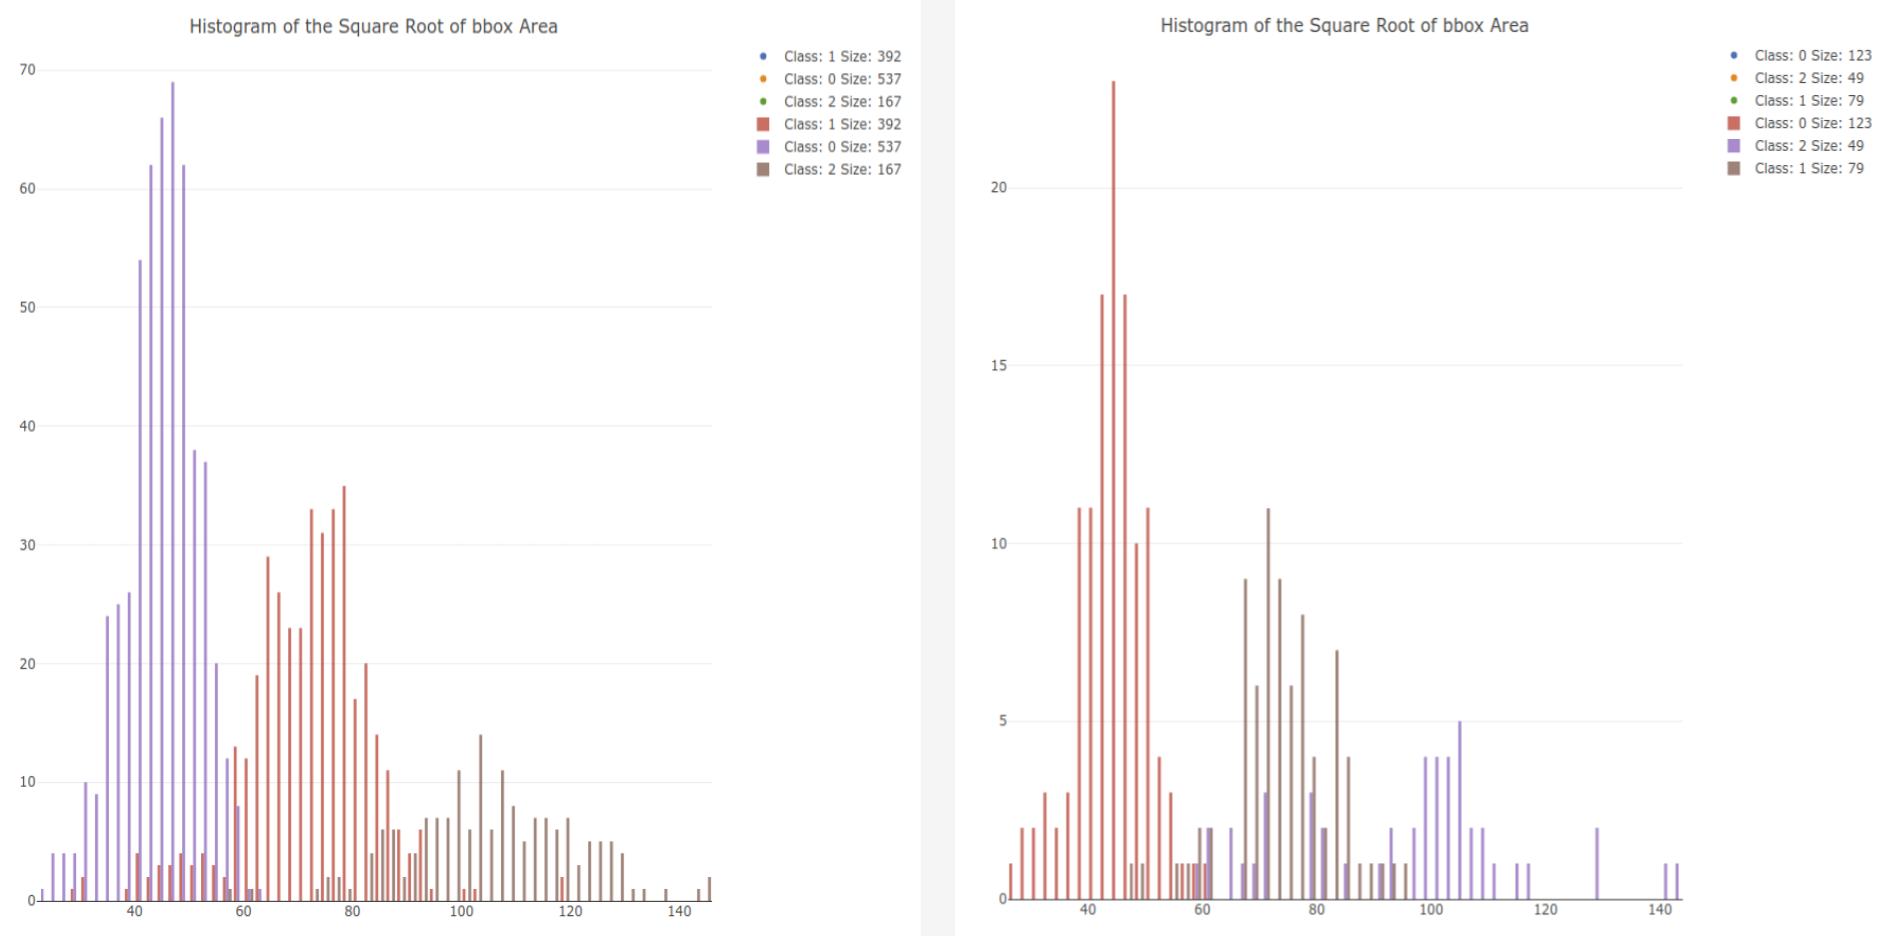
\includegraphics[width=1.0\textwidth]{Figures/SealStats.png}
\caption{}
\label{fig:SealStats}
\end{figure}

%
% % Of course, if you prefer, you can just start with
% %   \chapter{My First Chapter Name}
% % and start typing away.
% \chapter{Just a Test}
% This is only a test.
% \section{A section}
% Lorem ipsum dolor sit amet, consectetuer adipiscing elit. Nulla odio
% sem, bibendum ut, aliquam ac, facilisis id, tellus. Nam posuere pede
% sit amet ipsum. Etiam dolor. In sodales eros quis pede.  Quisque sed
% nulla et ligula vulputate lacinia. In venenatis, ligula id semper
% feugiat, ligula odio adipiscing libero, eget mollis nunc erat id orci.
% Nullam ante dolor, rutrum eget, vestibulum euismod, pulvinar at, nibh.
% In sapien. Quisque ut arcu. Suspendisse potenti. Cras consequat cursus
% nulla.
%
% \subsection{A Figure Example}
% \label{ssec:figure_example}
%
% This subsection shows a sample figure.
%
% \begin{figure}[h]
%   \centering
%   \includegraphics[width=0.5\textwidth]{sandiego}
%   \caption[A picture of San Diego. Short figure caption must be \protect{$< 4$} lines in the list of figures]
% {A picture of San Diego.  Short figure caption must be \protect{$< 4$} lines in the list of figures and match the start of the main figure caption verbatim. Note that figures must be on their own line (no neighboring text) and captions must be single-spaced and appear \protect\textit{below} the figure.  Captions can be as long as you want, but if they are longer than 4 lines in the list of figures, you must provide a short figure caption.\index{SanDiego}}
%   \label{fig:sandiego}
% \end{figure}
%
% \subsection{A Table Example}
%
% While in Section \ref{ssec:figure_example} Figure \ref{fig:sandiego} we had a majestic figure, here we provide a crazy table example.
%
%
% %%%% TABLE 1 %%%%
% \vspace{0.25in}
% \begin{table}[!ht]
% \caption[A table of when I get hungry.  Short table caption must be \protect{$< 4$} lines in the list of tables]{A table of when I get hungry. Short table caption must be \protect{$< 4$} lines in the list of tables and match the start of the main table caption verbatim.  Note that tables must be on their own line (no neighboring text) and captions must be single-spaced and appear \protect\textit{above} the table.  Captions can be as long as you want, but if they are longer than 4 lines in the list of figures, you must provide a short figure caption.}
%
% \vspace{-0.25in}
% \begin{center}
% \begin{tabular}{|p{1in}|p{2in}|p{3in}|}
%
% \hline
% Time of day & Hunger Level & Preferred Food \\
%
% \hline
% 8am & high & IHOP (French Toast) \\
%
% \hline
% noon & medium & Croutons (Tomato Basil Soup \& Granny Smith Chicken Salad) \\
%
% \hline
% 5pm & high & Bombay Coast (Saag Paneer) or Hi Thai (Pad See Ew) \\
%
% \hline
% 8pm & medium & Yogurt World (froyo!) \\
%
% \hline
% \end{tabular}
% \end{center}
% \label{tab:analysis3}
% \end{table}



%% APPENDIX
% \appendix
% \chapter{Final notes}
% What to do about things \cite{Martin_1983}.  What did he say \cite{Rilling_Insel_1999}.
%   Remove me in case of abdominal pain.



%% END MATTER
% \printindex %% Uncomment to display the index
% \nocite{}  %% Put any references that you want to include in the bib
%               but haven't cited in the braces.
% \bibliographystyle{alpha}  %% This is just my personal favorite style.
%                              There are many others.
%\setlength{\bibleftmargin}{0.25in}  % indent each item
%\setlength{\bibindent}{-\bibleftmargin}  % unindent the first line
%\def\baselinestretch{1.0}  % force single spacing
%\setlength{\bibitemsep}{0.16in}  % add extra space between items
% \bibliography{main}  %% This looks for the bibliography in template.bib
\printbibliography[heading=bibintoc]
%                          which should be formatted as a bibtex file.
%                          and needs to be separately compiled into a bbl file.
\end{document}
